% !TEX encoding = UTF-8 Unicode
%%%%%%%%%%%%%%%%%%%%%%%%%%%%%%%%%%%%%%%%%%%%%%%%%%%%%%%%%%%%%%%%%%%%%%%%%%%%%%%%%%%%%%%%%%%%%%%%%%%%%%% 
%%
%%  This file is asmeconf-template.tex, a LaTeX template to format ASME Conference papers according to
%%  the requirements on ASME's conference web pages, and including hypertext support for the pdf.
%%
%%  This file is version 1.34 dated 2022/12/30
%%  
%%  As of version 1.11, this template defaults to ASME's newer conference guidelines first posted July 2019.
%% 			Those guidelines changed the requested author block formatting to be inline. 
%%			This LaTeX template continues to support the traditional grid format as a package option, [grid].
%%			Nomenclature now follows the abstract. Abstract text is set in italics.
%%
%%  Author: John H. Lienhard V
%%          Department of Mechanical Engineering
%%          Massachusetts Institute of Technology
%%          Cambridge, MA 02139-4307 USA
%%
%%  Class options include:
%%
%%          * Math options from M. Sharpe's newtxmath package: upright integrals [upint]; 
%%          *    [varvw] for a v and w that are better distinguished from Greek nu; and also 
%%          *    [subscriptcorrection, smallerops, varg, frenchmath, varbb, cmbraces, slantedGreek,...] 
%%			* 	 See newtx documentation for descriptions (at CTAN: http://ctan.org, v1.6 or higher is best).
%%
%%          * Options to: 	omit the ASME copyright footer [nofoot]; 
%%			*				use government employee copyright notice [govt];
%%			*				use government contractor copyright notice [contractor]
%%
%%          * An option to use the traditional grid arrangement of author names [grid].  
%%			*	 With this option, line breaks (\\) may be inserted into the address as needed. 
%%			*	 Author names that include commas should be enclosed in braces, e.g., {Joseph L. Smith, Jr.}.  
%%			*	 Authors may be grouped above a single affiliation using braces, e.g., {Henry Tudor, Catherine Parr}.
%%
%%          * An option to balance the heights of columns on the last page [balance]. 
%%          *    This option is NOT compatible with the [lineno] option.
%%
%%          * An option to include line numbers [lineno]. You must *run twice* for proper placement of the line numbers. 
%%			*	 The lineno package does not number titles, footnotes, captions, or tables.
%%          *    This option will disable balancing column height on final page if that option has been invoked.
%%          *    The lineno package won't always number the lines preceding displayed math in a paragraph because
%%          *    paragraph has not ended.  See that package's documentation for macros to address this problem, or
%%          *    just leave a blank line above the displayed equation while you are editing and then remove the 
%%          *    blank line and [lineno] option when you move to your final version.
%%
%%			* Options for PDF/A compliance. [pdf-a] will produce PDF/A-3u compliance with sRGB OutputIntent.
%%			*	 [pdfapart= 1 or 2 or 3] and [pdfaconformance= b or u] can enable levels 1b, 2b, 2u, and 3b.
%%			*    The most recent versions of LaTeX (2021 and later) are moving toward integrated support for pdf-a, 
%%			*    through \DeclareDocumentMetadata{..}. The asmeconf class supports these new features, which can 
%%			*	 replace the aforementioned class options. (An up-to-date LaTeX installation is required to use this.)
%%
%%          * Many options for calligraphic, script, and fraktur fonts from the mathalfa package; the
%%          *    example shown here is: [mathalfa=cal=boondoxo] to use a Boondox font for \mathcal.
%%          *    Some other options for cal are: dutchcal, zapfc, cm (default), euler,...
%%          *    frak (fraktur), bb (blackboard bold), scr (script) may also be chosen this way.
%%			*	 For details, refer to mathalfa documentation (at CTAN: http://ctan.org).
%%
%%          * Option to use superiors font from newtxtext for footnotes [nodefaultsups] and
%%          *    for slightly larger small capitals, [largesc], also from newtxtext.
%%
%%          * An option to allow hyphenation of the typewriter font [hyphenate], from inconsolata package.
%%          *    Hyphenation is normally suppressed for typewriter mode because it is often used for code.
%%			*	 To replace the default variable word spacing by monospacing, use the option [mono].
%%			*	 To get a zero without a slash, use [var0]
%%
%%          * Options (used by the babel package) to include passages in languages other than English (e.g., a translation 
%%			*    of the abstract). Languages are called as options, e.g. [french], [spanish], [greek], [russian], etc. 
%%			*    Language support is greatest when running LuaLaTeX with the [fontspec] option.
%%			*    See Appendix B for details.
%%
%%  The use of commands defined or modified by the asmeconf class is illustrated throughout this file. In particular, 
%%  ASME requires capitalized, sans-serif section headings, and as a result some care is needed when using macros 
%%  in section headings, as also illustrated below.
%%
%%  Use an up-to-date and complete installation of LaTeX, such as TeX Live 2020 or later. Errors may occur with old set-ups.
%%
 %=========================================================
%% 
%% LICENSE: 
%%
%% Copyright (c) 2022 John H. Lienhard
%%
%% Offered under the MIT license: https://ctan.org/license/mit 
%%
%%%%%%%%%%%%%%%%%%%%%%%%%%%%%%%%%%%%%%%%%%%%%%%%%%%%%%%%%%%%%%%%%%%%%%%%%%%%%%%%%%%%%%%%%%%%%%%%%%%%%%% 

%% New pdf management code (June 2021); with this, the class option [pdf-a] can be omitted.
%% This change to the LaTeX kernel is being phased-in by the LaTeX3 team. Can delete if it gives you trouble.
%% Under LuaLaTeX, choose pdfstandard=A-3b (and be cautious when loading extra fonts)

%\DocumentMetadata{%
%	pdfstandard=A-3b,% A-2b, A-2u, A-3b, or A-3u
%	pdfversion=1.7,
%	lang=en-US,
%}

%%%%%%%%%%%%%%%%%%%%%%%%%%%%%%%%%%%%%%%%%%%%%%%%%%%%%%%%%%%%%%%%%%%%%%%%%%%%%%%%%%%%%%%%%%%%%%%%%%%%%%%

%% Class options are described above. Change these options as desired. 
%%		If you are not using the language options, remove them (together with Appendices B and C)
%%	 	Remove the [colorlinks] option before *final* submission to ASME, to get black text for printing,
%%		but keep that option for other uses.
 
\documentclass[balance,upint,subscriptcorrection,varvw,mathalfa=cal=boondoxo,spanish,french,vietnamese,russian,greek,pdf-a,colorlinks]{asmeconf}

%%%%%  pdf metadata  %%%%%%%%%%%%%%%%%%%%%%%%%%%%%%%%%%%%%%%%%%%%%%%%%%%%%%%%%%%%%%%%%%%%%%%%%%%%%%%%%%

\hypersetup{%
	pdfauthor={John H. Lienhard},
	pdftitle={MDO Final Report},                  % <=== change to YOUR pdf file title
	pdfkeywords={Multi-Disciplinary Design Optimization, Carbon Sequestration},% <=== change to YOUR pdf keywords
	pdfsubject = {Multi-Disciplinary Design Optimization},			  % <=== change to YOUR subject
%	pdfurl={https://ctan.org/pkg/asmeconf},% may delete
% pdflicenseurl={https://ctan.org/pkg/asmeconf},% may delete
}

%%%%%%%%%%%%%%%%%%%%%%%%%%%%%%%%%%%%%%%%%%%%%%%%%%%%%%%%%%%%%%%%%%%%%%%%%%%%%%%%%%%%%%%%%%%%%%%%%%%%%%%

\begin{document}

% Change these fields to the right content for your conference.
% You can comment these out if for some reason you don't want a header.
% Use title case (first letters capitalized), not all capitals

\ConfName{Presented to the MDO teaching team 2023\linebreak In Partial Fulfillment Of the Requirements for the Course\linebreak 16.888 MDO; Multidisciplinary Design Optimization
}
%\ConfAcronym{IMECE2023}
\ConfDate{Feburary - May 2023} % update 
\ConfCity{Cambridge, MA} % update 
%\PaperNo{IMECE2023-XXXX}

% Units of measure (e.g., cm) and other specialty lowercase terms in the title should be 
%   enclosed in \NoCaseChange{...} to maintain lower case type
%   LaTeX will automatically set the rest of the title in all capital letters.

\title{Terra Sparkling: Multi-Disciplinary Design Optimization for Carbon Sequestration} % <=== replace with YOUR title
%\title{Place Title Here: Place Subtitle After Colon} 
 
%   Put author names into the order you want. Use the same order for affiliations.
%   \affil{#} tags the author's affiliation to the address in \SetAffiliation{#}.
%   No space between last name and \affil{#}, separate names with commas.
%
%	For a sole author or a single affiliation for all authors, {#} may be left empty, as \affil{} and \SetAffiliation{} (but not with [grid] option!)
%
%   \CorrespondingAuthor{email} follows that author's affiliation, no spaces.  
%   If multiple corresponding authors, put both email addresses in the same command and place after both authors.
%
%   \JointFirstAuthor, if applicable, follows the affiliation of the relevant authors, no spaces.

\SetAuthors{%
        Warren Anderson\affil{1},
        John Beilstein\affil{1},
        Brooke DiMartino\affil{1},
        Tanner Papenfuss\affil{1},
        Stephen Tainter\affil{1}
	% John H.\ Lienhard\affil{1}\JointFirstAuthor\CorrespondingAuthor{}, 
	% Luis Hern\'andez\affil{2}\JointFirstAuthor, 
	% Maria Silva\affil{3}, 
	% Henry Tudor\affil{4},  
	% Catherine~Parr\affil{4}\CorrespondingAuthor{lienhard@mit.edu, kate@thepalace.gov}
	}

\SetAffiliation{1}{Massachusetts Institute of Technology, Cambridge, MA }
%\SetAffiliation{2}{Institution or Company Name, City, State}
%\SetAffiliation{3}{Institution or Company Name, City, Province, Canada}
%\SetAffiliation{4}{Hampton Court Palace, Richmond, England}
%	Note: Luis and Maria are not real people.  Henry and Catherine have been dead for >450 years.

%	To switch from inline author names to gridded names, use the [grid] option.

\maketitle

%%% Use this footnote for tracking various versions of your draft. Change text to suit your own needs. 
%%% \date{..} calls the same command. 
%\versionfootnote{Documentation for \texttt{asmeconf.cls}: Version~\versionno, \today.}% <=== Delete before final submission.

%%% Change these to your keywords.  Keywords are automatically printed at the end of the abstract.
%%% This command MUST COME BEFORE the end of the abstract.
%%% If you don't want keywords, leave the argument of \keywords{} empty (or use the abstract* environment)

\keywords{Multi-Disciplinary Design Optimization, CCUS, Carbon Sequestration}

%%%%%  End of fields to be completed. Now write your paper. %%%%%%%%%%%%%%%%%%%%%%%%%%%%%%%%%%%%%%%%%%%


%%%%%  ABSTRACT  %%%%%%%%%%%%%%%%%%%%%%%%%%%%%%%%%%%%%%%%%%%%%%%%%%%
%%
%% Abstract should be 200 words or less
\begin{abstract}
[TO DO. FILL IN THE ABSTRACT AT THE END.]
%This paper is an example of and a  {\upshape\LaTeX} template for typesetting ASME conference papers using the {\upshape\texttt{asmeconf}} class. This  {\upshape\LaTeX} template follows ASME guidelines for margins, fonts, headings, captions, and reference formats as of 2022. The class is intended to be used with the {\upshape\texttt{asmeconf.bst} \hologo{BibTeX}} style for reference formatting, which is part of this distribution. The template produces pdfs that contain hyperlinks, bookmarks, and metadata; and references can include the DOI and URL fields. Links may be colored, for online use, or black, for publication. The class enables inline author names, following ASME's current style, but can also produce the traditional grid style. Options include line numbering, final column balancing, various math options, government copyright, and archivability (PDF/A). In addition, section headers may contain mathematics, references, citations, and footnotes. The class is compatible with {\upshape\hologo{pdfLaTeX}} or {\upshape\hologo{LuaLaTeX}}.
\end{abstract}

%%%%%%%%%  NOMENCLATURE (OPTIONAL) %%%%%%%%%%%%%%%%%%%%%%%%%%%%%%%%%
%%
%% To change space between the symbols and  definitions, use \begin{nomenclature}[Xcm] where X is a number 
%% The unit cm can be replaced by any LaTeX unit of dimension: pt, in, ex, em, pc, etc.
%% Default is 2em.
%% \EntryHeading{..} produces an italicized subheading in the nomenclature list, e.g., \EntryHeading{Greek letters}

% \begin{nomenclature}
% \EntryHeading{Roman letters}
% \entry{$k$}{Thermal conductivity [W m$^{-1}$ K$^{-1}$]}
% \entry{$\vec{q}$}{Heat flux vector [W m$^{-2}$]}

% \EntryHeading{Greek letters}
% \entry{$\alpha$}{Thermal diffusivity [m$^2$ s$^{-1}$]}
% \entry{$\nu$}{Kinematic viscosity [m$^2$ s$^{-1}$]}

% \EntryHeading{Dimensionless groups}
% \entry{Pr}{Prandtl number, $\nu/\alpha$}
% \entry{Sc}{Schmidt number, $\nu/\mathcal{D}_{1,2}$}

% \EntryHeading{Superscripts and subscripts}
% \entry{b}{bulk value}
% \entry{$\infty$}{free stream value}
% \end{nomenclature}

%%%%%%%%%  BODY OF PAPER %%%%%%%%%%%%%%%%%%%%%%%%%%%%%%%%%

\section{Introduction and Motivation}
CO2 makes up 80\% of greenhouse gas emissions in the US, and its accumulation in the atmosphere is a leading cause of global warming. CO2 is the primary greenhouse gas emitted by anthropogenic sources and according to OurWorldInData.org, humanity produced 37.1 billion tons of carbon dioxide emissions in 2021. ~46\% of US CO2 emissions are produced by electricity generation and industries that use fossil fuel or produce CO2 through chemical reactions (i.e., cement, steel, and petrochemical plants). \cite{EPA_2017}

One promising solution to this problem is utilizing Point-Source Capture (PSC) and permanently storing it underground in a process called sequestration. The technology of injecting CO2 into the subsurface is nothing new; oil companies have injected CO2 into depleted hydrocarbon reservoirs for enhanced recovery for decades. It is important to note that this enhanced recovery does little to impact the overall CO2 emissions into the atmosphere, but it does prove that permanent sequestration is technically possible. Two pilot programs in the US were primarily funded by the Department of Energy that tested aspects of CO2 sequestration at a commercial scale. The Petra Nova project, located southwest of Houston, Texas, took CO2 captured from an electric generation station and piped it 81 miles to the West Ranch Oil Field for enhanced oil recovery \cite{Smyth2020}. The Illinois Basin Decatur Project is the second project, and it has successfully injected 1.3 million metric tons of CO2 \cite{IBDP2017}.

\section{Opportunity}
Between 2021 and 2022, an estimated 78 new US carbon capture utilization and storage (CCUS) projects were announced \cite{CCSProjects2023}. While the number of CCUS projects in the planning and evaluation phases has been rising recently, there has been a significant increase in the last year due to the Inflation Reduction Act of 2022 (IRA). Previously the 45Q tax code credited \$50/ton of CO2 that was captured and stored using PSC. With the IRA, the credit has been raised to \$85/ton for PSC-based CCUS projects. This credit value increase has a lot of companies seriously looking at ways to make a commercial-scale CCUS plant viable \cite{IRA2022}. 

Due to the capital investment that would be required, even with the IRA credit at \$85/ton of CO2, the margins for making CCUS profitable are going to be narrow. Every function within a total PSC to CCUS system must be optimized for efficiency and cost. This paper uses a multidisciplinary approach to optimize the objectives through simulation and modeling, representing real-world scenarios as closely as possible. 

In 2013 the USGS conducted a CO2 storage resource assessment of the US for potential CCUS reservoirs \cite{USGS2013}. According to their finding, the Coastal plains of Texas, Louisiana, Mississippi, Alabama, and the Florida panhandle have a potential storage capacity of 1,900 Gt of CO2 or about 65\% of all US capacity. This area is also densely populated with electric generation and petrochemical plants, so this region was a prime candidate for this PSC to CCUS optimization problem.

\section{Problem Formulation}
The purpose of this project is to design a system that maximizes the project Net Present Value (NPV) and minimizes the amount of CO2 generated by the point-source compression to supercritical conditions for transportation and injection into the subsurface. The model cumulative injection cannot exceed the reservoir volume capacity, nor can the injection pressure at the bottom of the wellbore exceed the maximum injection pressure set by the pore pressure fracture gradient. These problem objectives and constraints are summarized in equations (1) and (2) below, respectively:
\begin{equation}
  min\ J(x) = 
  \begin{pmatrix}
      -Net\ present\ value,\ NPV \\
      CO2\ generated,\ tot\_CO2\_gen
  \end{pmatrix}
\end{equation}
\begin{equation}
  s.t.\ g(x) = 
  \begin{pmatrix}
      q_{inj} * num\_wells * time-res\_volume \\
      p_{wellbore} - p_{max\_injection}
  \end{pmatrix}
  \leq 0
\end{equation}

For the design, the team chose to focus on nine key variables. These are summarized in the Master Table, figure \ref{master_table:1}, along with the parameters used to build the model. Because all modules are being built from the ground up, there are many parameters included in our problem. It is worth noting that the problem has been simplified in several key ways:
\begin{enumerate}
  \item The system assumes steady-state conditions, constant across the project's life.
  \item The subsurface has been simplified to Darcy's Law, with no change to reservoir pressure over time.
  \item All compression calculations assume diesel as the fuel type.
  \item If there are multiple facility tie-ins, it assumes they all converge to one processing facility before entering our system.
  \item No downtime is considered for the system over the 20-year period it is online.
\end{enumerate}

%%%%%%%%%%%%% begin figure %%%%%%%%%%%%%%%%%
%% captions go below figures
\begin{figure*}[btp]
\centering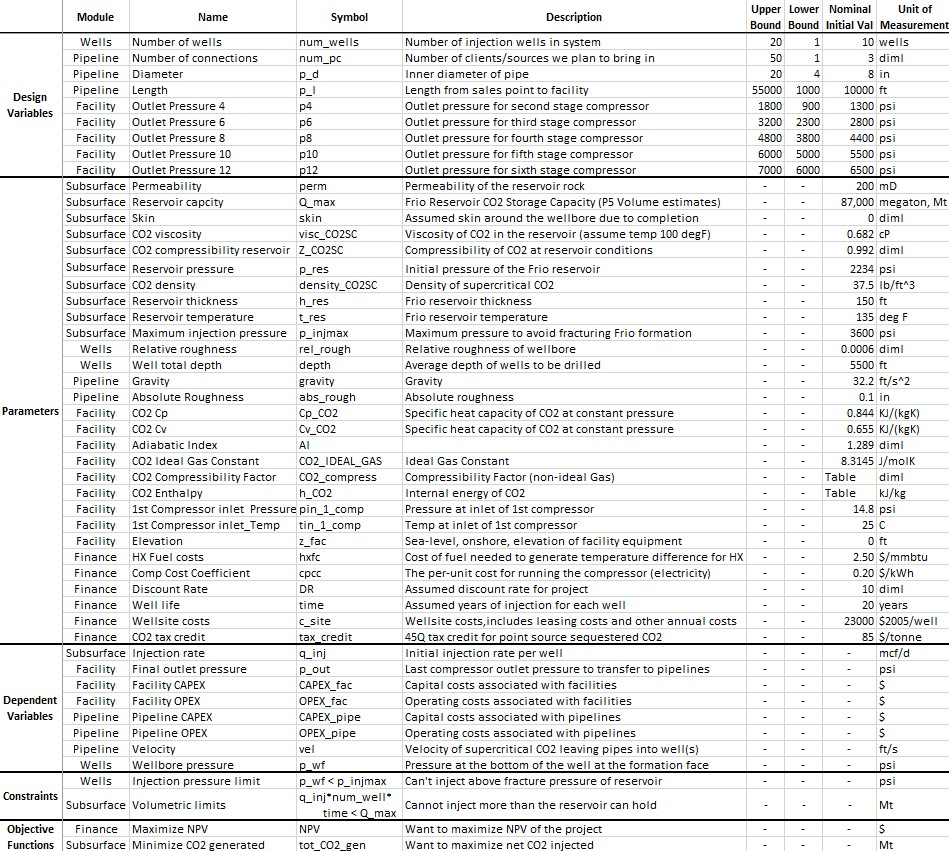
\includegraphics[width=0.95\linewidth]{images/Master_Table_v4.jpg}
\caption{Master Table of design variables, parameters, dependent variables, constraints, and objectives }\label{master_table:1}
\end{figure*}
 %%%%%%%%%%%%% end figure %%%%%%%%%%%%%%%%%%%

\section{Modeling and Simulation}
\subsection{Modules} 
Each module was separately modeled per the block diagram (Appendix A) and N2 diagram (Appendix B) with standardized coupled variables, which allowed the team to develop the models of each module in parallel and with some modeler autonomy in the equations and techniques used.

\subsubsection{Facilities}
The Facilities module comprised of the release of \begin{math}{CO_2} \end{math} from the sorbent in a point-source capture system, to the outlet of the point-source physical footprint such that the \begin{math}{CO_2} \end{math} has reached a supercritical state before transport in the Pipeline Module. 
Based on the paper from Jackson et. Al 2018 \cite{jackson_2018}, the team developed equations to represent the changes from the start point to end-state (super critical point). As seen in Figure \ref{enthalpy_diagram:1} and \ref{comphx:1} below, the design of the facilities section considers stages of compressors and heat exchangers to work up from the start point up to the supercritical point. The module uses the design variables to find the most ‘energy efficient pathway’ to the supercritical point. The advantage of operating a CCUS system in a supercritical state is that \begin{math}{CO_2} \end{math} has the density of a liquid, but retains the viscosity of a gas, which enables the system to process \begin{math}{CO_2} \end{math} in a more capitally efficient manner. 

%%%%%%%%%%%%% begin figure %%%%%%%%%%%%%%%%%
%% captions go below figures
\begin{figure*}[h!t]
\centering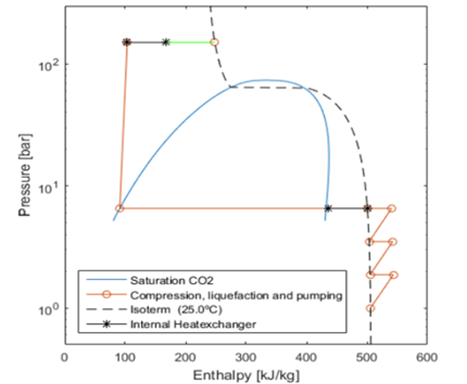
\includegraphics[width=0.25\linewidth]{images/enthalpy_diagram.png}
\caption{Compress and cool \begin{math}{CO_2} \end{math} to a supercritical state}\label{enthalpy_diagram:1}
\end{figure*}
 %%%%%%%%%%%%% end figure %%%%%%%%%%%%%%%%%%%

%%%%%%%%%%%%% begin figure %%%%%%%%%%%%%%%%%
%% captions go below figures
\begin{figure*}[h!t]
\centering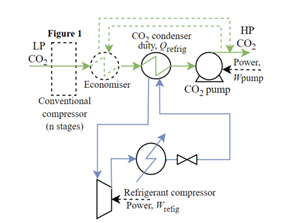
\includegraphics[width=0.25\linewidth]{images/compression-hx.png}
\caption{Compressor and heat exchanger layout for each stage in Figure \ref{enthalpy_diagram:1}}\label{comphx:1}
\end{figure*}
 %%%%%%%%%%%%% end figure %%%%%%%%%%%%%%%%%%%

To model \begin{math}{CO_2} \end{math} behavior through a compressor, a polytropic behavior was assumed, and the equation (3) seen below was used. This equation calculates the work required to compress the \begin{math}{CO_2} \end{math} from an inlet state \begin{math}{i} \end{math} to the outlet state \begin{math}{j} \end{math}. The volume and temperature anticipated at the outlet can be calculated using the formula (4) and (5). 

\begin{equation}
    \dot{W}_{ij} = p_i \dot{v_i} \frac{\dot{v_j}^{1-n}-\dot{v_i} ^{1-n}}{1-n} 
\end{equation}

\begin{equation}
    \dot{v}_j = \bigg(\frac{p_i \dot{v_i}^n}{p_j}\bigg)^\frac{1}{n} 
\end{equation}

\begin{equation}
    T_j = \bigg(\frac{p_j}{p_i}\bigg)^\frac{n-1}{n} 
\end{equation}

Next, per Figure \ref{enthalpy_diagram:1}, the \begin{math}{CO_2} \end{math} is cooled to 25$^{\circ}$C before entering the next stage, while maintaining the same pressure from the outlet of the compressor. Thus, the heat required to cool the system can be calculated as follows.

\begin{equation}
    \dot{Q}_{ij} = \dot{m} \big(h_j-h_i)
\end{equation}

\begin{equation}
    \Delta h_{ij} = c_p\big(T_j-T_i)
\end{equation}

Once the energy requirements have been determined for one stage, this is repeated in series seven times per Jackson et. Al 2018 \cite{jackson_2018}, until the \begin{math}{CO_2} \end{math} reaches a supercritical state. 
After calculating the energy required for each stage, the costs for delivering that energy can be modeled as well. To do so, each of the unitized energy calculations must be multiplied by the mass flow rate of the system. The team utilized various research papers that parameterized capital (CAPEX) and operating (OPEX) costs for compressors and heat exchangers. Referencing Darrow et. Al 2015 \cite{darrow}, the capital and operating costs for a compressor can be seen below:

\begin{equation}
    W_{ij_{CAPEX}} = \frac{\$2020.6}{kWh}W_{ij}
\end{equation}

\begin{equation}
    \begin{array}{l}
        W_{ij_{OPEX}} = \frac{365 days}{year}\bigg(\frac{\$3.06}{MMBTU}*\frac{1 MMBTU}{293.07 kWh} \\
        + \frac{24 hrs}{day}*\frac{\$0.01108}{kW}\bigg)W_{ij}
    \end{array}
\end{equation}

In the OPEX equation, it is important to note that there are fuel costs, and O\&M costs. 

Similarly for the heat exchanger, the CAPEX and OPEX equations originated from Bautista 2014 \cite{bautista}. 

\begin{equation}
    Q_{ij_{CAPEX}} = \frac{\$247.35}{kWh}Q_{ij}
\end{equation}

\begin{equation}
    Q_{ij_{OPEX}} = Q_{{elec}_{OPEX}} + Q_{{refrig}_{OPEX}} + Q_{{water}_{OPEX}}
\end{equation}

\begin{equation}
    Q_{{elec}_{OPEX}} = \frac{\$75.66/kWh_{elec}}{kWh_{cooled}}Q_{ij}
\end{equation}

\begin{equation}
    Q_{{refrig}_{OPEX}} = \frac{\$0.009/kWh_{ref}}{kWh_{cooled}}Q_{ij}
\end{equation}

\begin{equation}
    Q_{{water}_{OPEX}} = \frac{\$0.0097/kWh_{m^3}}{kWh_{cooled}}Q_{ij}
\end{equation}

In addition to calculating costs, the emissions generated with the compression (fuel emissions) and cooling (electricity grid intensity) were calculated to understand how much \begin{math}{CO_2} \end{math} was generated in this process.

\begin{equation}
    CO_{2_{W_{ij}}} = CO_{2_{fuel}}W_{ij}*24*365
\end{equation}

\begin{equation}
    CO_{2_{HX_{ij}}} = \frac{Elec_{HX_{ij}}*CO_{2_{TX_{grid}}}}{1000}*24*365
\end{equation}

\begin{equation}
    Elec_{HX_{ij}} = \frac{757.28*CO_{2_{TX_{grid}}}}{1000}*24*365
\end{equation}

\begin{equation}
    CO_{2_{TX_{grid}}} = \frac{941 lb}{MWh}*\frac{0.453 kg}{lb}
\end{equation}

Each cost and emission value from each stage were then aggregated to calculate the total costs and emissions across the entire and routed to the Finance module.

\subsubsection{Pipelines}

The pipeline module takes the final supercritical pressure state from the Facilities module and calculates the pressure drop across the distance of the pipeline. When CO2 drops below the supercritical state, a booster pump is installed to return the CO2 to a supercritical state. 

Pressure drop is determined by multiple factors such as pipe length and diameter, but it also leverages the fanning coefficient, which calculates the estimated frictional effects using pipe diameter and the Reynolds number (Neutrium).  Since the viscosity used for the Reynolds number can change with state conditions of the CO2, the viscosity is a dynamic formula based on temperature changes (Nave).

\begin{equation}
    \Delta p = 2f\rho_{new}v^2\frac{length_{pipe}}{diameter_pipe}
\end{equation}

\begin{equation}
    \frac{1}{\sqrt{f}} = -2\log_{10}\Bigg(\frac{\epsilon/D}{3.7065}-\frac{5.0452}{Re}\log_{10}\bigg(\frac{{\epsilon/D}^{1.1098}}{2.8257}+\frac{5.8506}{Re^{0.8981}}\bigg)\Bigg)
\end{equation}

\begin{equation}
    \upsilon = \upsilon_0\bigg(\frac{a}{b}\bigg)\bigg[\frac{T}{T_0}\bigg]
\end{equation}

\begin{equation}
    \begin{array}{l}
        a = 0.555T_0+C \\
        b = 0.555T+C
    \end{array}
\end{equation}

Costs and emissions associated with the pipeline and compressors leverage the equations below and equations used in the Facilities module.

\begin{equation}
    CAPEX_{pipeline} = \bigg(32.086p_ln_{pc}^{-0.033p_d}\bigg)p_l n_{pc}
\end{equation}

\subsubsection{Wells}

Once the CO2 has been delivered from the point source to wellhead, the Wells module calculates the pressure at the reservoir face at the end of the well. Similar to the pipeline module, the well transports the CO2 vertically into the ground through tubing which can be modeled as a pipe. 

\begin{equation}
    p_{wf}(t) = p_{wh}-\Delta p_f + \rho gD
\end{equation}

\begin{equation}
    f = 0.0055\bigg(1+\bigg(2*10^4\frac{k}{D}+\frac{10^6}{Re}\bigg)^{\frac{1}{3}}\bigg)
\end{equation}

\begin{equation}
    \Delta P_f = \frac{2f\rho v^2L}{g_cD}
\end{equation}

\begin{equation}
    Re = \frac{1988\rho VD}{\mu}
\end{equation}

The cost per well can be seen below:

\subsubsection{Subsurface}

The Subsurface module then determines the volumetric flowrate of CO2 entering the reservoir given the bottom hole pressure derived from the Well module, and the static reservoir pressure. The formula used below is derived from reservoir engineering principles for a gas injection well (NEED SOURCE).

\begin{equation}
    q_g = \frac{0.703kh(p_{R}^{2}-p_{wf}^{2})}{T\mu_{g}Z[ln(\frac{r_e}{r_w})-0.75+s]}
\end{equation}


While this module was simplified in terms of fluid dynamics and geomechanics given the time constraints of the class, a constraint was applied to ensure that the total volume injected doesn’t exceed the total volume of the target reservoir. The target reservoir was estimated to have a volume of XXXXXXXXXXX, determined by estimating the pore volume of XXXXXXXXXX reservoir that research has identified as a suitable target (how did you pick the reservoir)
The equation for calculating pore volume



\subsubsection{Finance}
The finance module ultimately provides the primary objective output: NPV. It calculates the revenue, total CAPEX, annual CAPEX, and annual OPEX to keep the system online over its lifetime. From this, it can calculate the upfront capital spend at time 0 along with the annual cashflow. The annual cashflow is then discounted and summed over the life of the project to generate the net present value. The critical equation for this module is as follows:
\begin{equation}
    NPV = \sum_{t=1}^{T} \frac{cashflow_t}{(1+discount\_rate)^t} - CAPEX_0
\end{equation}

\subsection{Validation}

The model was initially validated by checking the deterministic output with a manual excel model and with research papers for similar orders of magnitudes of results. The initial design vector \begin{math}{x_0} \end{math} was pulled from our design-of-experiments (DoE).

%%%%%%%%%%%%% begin table %%%%%%%%%%%%%%%%%
\begin{table}[h!]
\caption[Table]{Design Vector \begin{math}{x_0} \end{math}}\label{x0:1}
\centering{%
\begin{tabular}{llr}
% \begin{tabular}{!{\hspace*{0.5cm}} >{\raggedright\hangindent=1em} p{3cm} d{3.3} @{\hspace*{1cm}} d{3.3} !{\hspace*{0.5cm}}}
\toprule
Design Variable & Value \\
\midrule
Num of Wells & 5 \\
Num of Connections &  2\\
Pipeline Diameter (in) &  12 \\
Pipeline Length (m) & 28000 \\
P2 (kPa) & 700 \\
P4 (kPa) & 1800 \\
P6 (kPa) & 3200 \\
P8 (kPa) & 4800 \\
P10 (kPa) & 5500 \\
P12 (kPa) & 7000 \\
\bottomrule
\end{tabular}
}
\end{table}

%%%%%%%%%%%%% end table %%%%%%%%%%%%%%%%%%%

%%%%%%%%%%%%% begin table %%%%%%%%%%%%%%%%%
\begin{table}[h!]
\caption[Table]{Output from Design Vector \begin{math}{x_0} \end{math}}\label{x0:1}
\centering{%
\begin{tabular}{llr}
% \begin{tabular}{!{\hspace*{0.5cm}} >{\raggedright\hangindent=1em} p{3cm} d{3.3} @{\hspace*{1cm}} d{3.3} !{\hspace*{0.5cm}}}
\toprule
Output Variable & Value \\
\midrule
Tot \begin{math} {CO_2} \end{math} gen MMT/yr & 4.37 \\
Net CO2 MMT/yr & 4.24\\
Wellbore inj Press (psi) & 1471.6 \\
Total Injection VOlume (MMscf/day) & 19.55 \\
NPV (\$) & 4989\\
Pipe Press Out (kPa) & 350 \\
Pipe Velocity output (m/s) & 60.25 \\
\begin{math} {CO_2} \end{math} entering plant (kg/yr) & 126144000 \\
\bottomrule
\end{tabular}
}
\end{table}

%%%%%%%%%%%%% end table %%%%%%%%%%%%%%%%%%%

Additionally, we ran validation checks against the constraints and bounds of the optimization problem against our DoE to ensure the design space was correctly upholding bounds and constraints of the problem. This was relatively easy to do as the computational time was >10ms.


\section{Design of Experiments}

Upon completing the assembly of our model and ensuring its functionality, we established a Design of Experiments. Initially, we defined the bounds for each variable; see table \ref{bounds:1}. This was defined based on the outcomes of our problem formulation analysis. From our bounds, we created a list of options for each parameter, as seen in figure \ref{doe_options:1}. Subsequently, we employed the pycubeDOE \footnote{https://pypi.org/project/pycubedoe/} Python function to develop a comprehensive Design of Experiments seen in figure \ref{full_doe:1}. Finally, we executed our entire Design of Experiments via our model, generating a set of initial baseline responses that served as a starting point for further optimization.

\subsection{Key Results}
\subsection*{Best options:}
DOE Option 4: NPV –> \$30.69M

DOE Option 6: NPV -> \$24.44M

\subsection*{Worst option:}
DOE Option 20: NPV -> -\$6,170M

\subsection{Insights}
The optimal choices entail fewer connections and a shorter pipeline length. Conversely, the suboptimal alternative involves a longer pipeline length combined with more connections.

%%%%%%%%%%%%% begin table %%%%%%%%%%%%%%%%%
\begin{table}[t]
\caption[Table]{Bounds}\label{bounds:1}
\centering{%
\begin{tabular}{llr}
% \begin{tabular}{!{\hspace*{0.5cm}} >{\raggedright\hangindent=1em} p{3cm} d{3.3} @{\hspace*{1cm}} d{3.3} !{\hspace*{0.5cm}}}
\toprule
Option & Lower Bound & Upper Bound \\
\midrule
Number of Wells & 5 & 20 \\
Number of Connections &  1 & 3 \\
Pipeline Diameter &  4 & 20 \\
Pipeline Length &  1000 & 55000 \\
p2 & 500 & 700 \\
p4 & 900 & 1800 \\
p6 & 2300 & 3200 \\
p8 & 3800 & 4800 \\
p10 & 5000 & 6000 \\
p12 & 6000 & 7000 \\
\bottomrule
\end{tabular}
}
\end{table}

%%%%%%%%%%%%% end table %%%%%%%%%%%%%%%%%%%

%%%%%%%%%%%%% begin figure %%%%%%%%%%%%%%%%%

%% captions go below figures

\begin{figure*}[btp]
\centering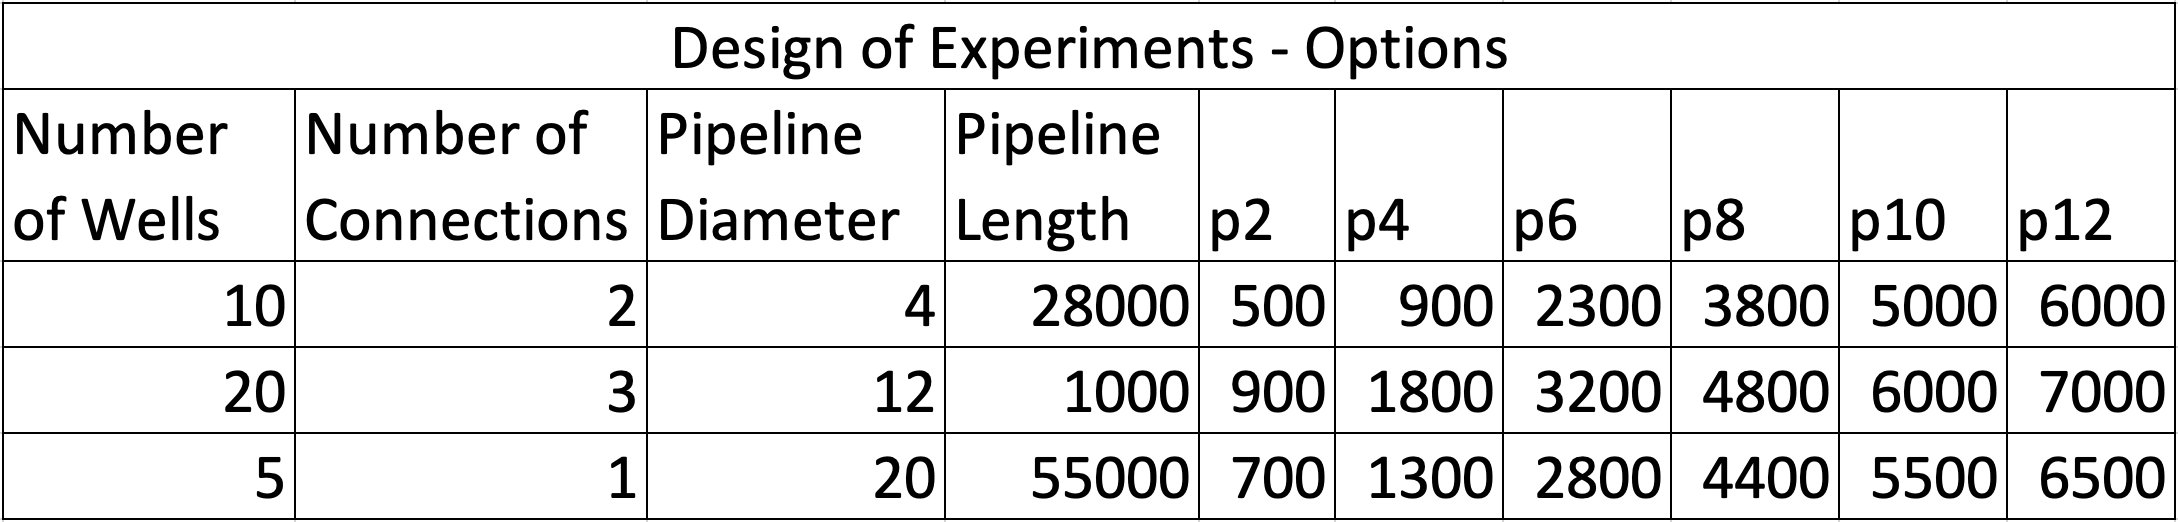
\includegraphics[width=0.7\linewidth]{images/DOE.png}
\caption{DOE Options}\label{doe_options:1}
\end{figure*}
 
%%%%%%%%%%%%% end figure %%%%%%%%%%%%%%%%%%%

%%%%%%%%%%%%% begin figure %%%%%%%%%%%%%%%%%

%% captions go below figures

\begin{figure}
\centering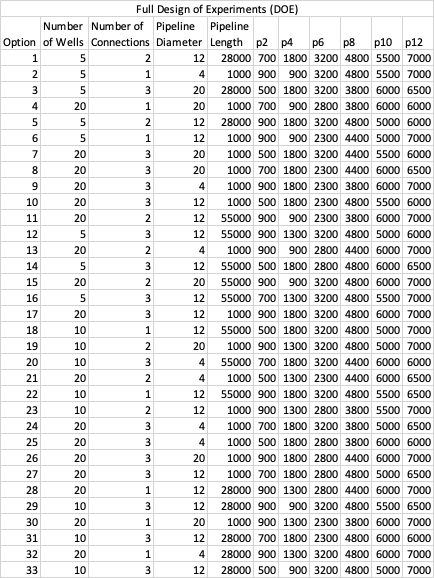
\includegraphics[width=0.7\linewidth]{images/full_DOE.png}
\caption{Full DOE Table}\label{full_doe:1}
\end{figure}
 
%%%%%%%%%%%%% end figure %%%%%%%%%%%%%%%%%%%

\section{Single Objective Optimization}
In this section, we will detail two efforts to optimize our model. First, we evaluated different gradient-based optimization algorithms. We ended up selecting a local derivative-free method due to the constraints of our model. Next, we tested several heuristic-based optimizations. Ultimately, we selected SLSQP and PSO for their respective advantages.

\subsection{Local derivative-free optimization}

Upon assessing the gradient-based optimization techniques we've learned, we concluded that our model's sheer number of equations would make it impractical to utilize such methods. Consequently, we explored the possibility of applying the "direct" approach for local derivative-free optimization. Unfortunately, we encountered issues implementing the algorithm using Python and could not achieve convergence toward a solution. Eventually, we opted for the Nelder-Mead method for local derivative-free optimization as a viable alternative. Figure \ref{nelder_option4:1} and \ref{nelder_option6:1} show the number of iterations for Nelder-Mead method convergence starting from DOE option 4 and option 6, respectively. Table \ref{nelder_convergence:1} shows the number of iterations and final NPV values for the same options. 

%%%%%%%%%%%%% begin figure %%%%%%%%%%%%%%%%%

%% captions go below figures

\begin{figure}
\centering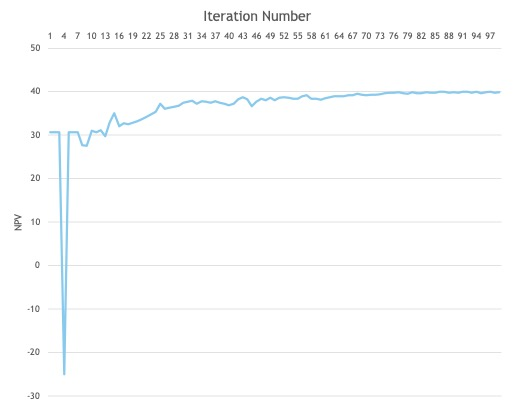
\includegraphics[width=0.7\linewidth]{images/nelder_option4.jpg}
\caption{Nelder-Mead Convergence Plot starting at DOE Option 4}\label{nelder_option4:1}
\end{figure}
 
%%%%%%%%%%%%% end figure %%%%%%%%%%%%%%%%%%%

%%%%%%%%%%%%% begin figure %%%%%%%%%%%%%%%%%

%% captions go below figures

\begin{figure}
\centering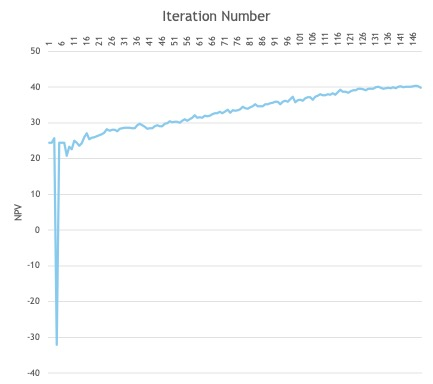
\includegraphics[width=0.7\linewidth]{images/nelder_option6.jpg}
\caption{Nelder-Mead Convergence Plot starting at DOE Option 6}\label{nelder_option6:1}
\end{figure}
 
%%%%%%%%%%%%% end figure %%%%%%%%%%%%%%%%%%%

%%%%%%%%%%%%% begin table %%%%%%%%%%%%%%%%%
\begin{table}[btp]
\caption[Table]{Nelder-Mead Convergence and NPV}\label{nelder_convergence:1}
\centering{%
\begin{tabular}{llr}
% \begin{tabular}{!{\hspace*{0.5cm}} >{\raggedright\hangindent=1em} p{3cm} d{3.3} @{\hspace*{1cm}} d{3.3} !{\hspace*{0.5cm}}}
\toprule
Starting point & Number of iterations to convergence & NPV \\
\midrule
DOE \#4 & 75 &  \$40.3M \\
DOE \#6 & 150 &  \$41.6M \\
\bottomrule
\end{tabular}
}
\end{table}

%%%%%%%%%%%%% end table %%%%%%%%%%%%%%%%%%%

\subsection{SLSQP and PSO}
After executing the Nelder-Mead algorithm, we experimented with various heuristic-based optimization algorithms. We selected two specific approaches: SLSQP (sequential least squares programming) and PSO (particle swarm optimization). Our rationale for choosing SLSQP was due to its speed and relative ease of implementation. On the other hand, we opted for PSO as it provided a more comprehensive set of tuning parameters for us to utilize. Figure \ref{optimization_4:1} and \ref{optimization_20:1} show the results of PSO and SLSQP starting at DOE options 4 and 20. 

%%%%%%%%%%%%% begin figure %%%%%%%%%%%%%%%%%

%% captions go below figures

\begin{figure*}[btp]
\centering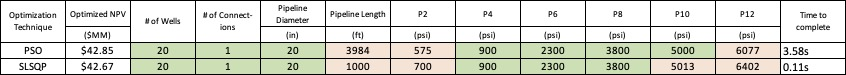
\includegraphics[width=0.7\linewidth]{images/optimization_point_4.jpg}
\caption{PSO and SLSQP table starting at DOE option 4}\label{optimization_4:1}
\end{figure*}
 
%%%%%%%%%%%%% end figure %%%%%%%%%%%%%%%%%%%

%%%%%%%%%%%%% begin figure %%%%%%%%%%%%%%%%%

%% captions go below figures

\begin{figure*}[btp]
\centering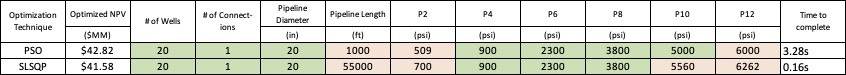
\includegraphics[width=0.7\linewidth]{images/optimization_point_20.jpg}
\caption{PSO and SLSQP table starting at DOE option 20}\label{optimization_20:1}
\end{figure*}

%%%%%%%%%%%%% end figure %%%%%%%%%%%%%%%%%%%

\subsection*{PSO tuning parameters}
The PSO algorithm has several tuning parameters. The two we focused on were the number of iterations and swarm size. Figures \ref{optimization_4:1} and \ref{optimization_20:1} were both run with a swarm size of 100 and iterations of 100. Table \ref{PSO_tuning:1} shows additional tuning parameters and their effect on the overall NPV. 

%%%%%%%%%%%%% begin table %%%%%%%%%%%%%%%%%
\begin{table}[!btp]
\caption[Table]{PSO Tuning}\label{PSO_tuning:1}
\centering{%
\begin{tabular}{llr}
% \begin{tabular}{!{\hspace*{0.5cm}} >{\raggedright\hangindent=1em} p{3cm} d{3.3} @{\hspace*{1cm}} d{3.3} !{\hspace*{0.5cm}}}
\toprule
Swarm Size & Number of Iterations & NPV \\
\midrule
100 & 100 &  \$43M \\
5 & 10 &  -\$24M \\
5 & 100 &  \$42M \\
100 & 5 &  \$40M \\
\bottomrule
\end{tabular}
}
\end{table}

%%%%%%%%%%%%% end table %%%%%%%%%%%%%%%%%%%
 


\section{Multi-Objective Optimization}
To implement the Multi-Objective Optimization (MOO) capabilities into our project we started off by investing several MOO frameworks that have been built in Python. We looked at a number of optimizer tools but ultimately settled on using PyMOO \cite{Blank2020}. We started off incorporating PyMOO by first creating a copy of both our Single Objective Optimizer (Optimzer_ldfo.py) and our experimentation module (Main.py). We then modified the Optimizer to incorporate a function call to the PyMOO plugin. We then modified the Main module (now called Main_MOO.py) to return two outputs (NPV and CAPEX). The new Main_MOO module was further updated to append to a .csv file specific information about each iteration through the optimizer. This information included the design vector requested by the optimizer, as well as the resulting NPV, CAPEX, CO2 generated, and CO2 injected. This allowed us to track the progress of the optimizer as it marched from an initial design vector starting point provided by the team towards its ultimate "optimal solution". 

Once the modules were updated to incorporate the PyMOO framework we decided to look at two methods of performing MOO's. The first was the Non-Dominated Sorting Genetic Algorithm (NSGA-2) and the second was the S-Metric Evolutionary Multi-Objective Optimization Algorithms (SMS-EMOA). 

As mentioned, the first method we used to analyze our problem set was the NSGA-2 method. This method involved importing the algorithm from the PyMOO framework and providing execution parameters for the algorithm to adhere to. Our team performed a small sensitivity analysis to better understand how changing these parameters affected the algorithm's optimal solution. We ultimately decided to investigate the solution results and number of iterations required to perform the algorithm based upon: population size, mutation rate, cutoff, and number of offspring. The results from this investigation can be seen in Figure \ref{NSGA:1}. After running the initial sensitivity analysis we decided to take the two best results, and combine them to see if the resulting parameters would yield a beneficial result. It turns out in this case that combining mutation rate and number of offspring did yield a better end result than changing any one single parameter. The number of iterations required to perform these calculations ranged between 1380 and 2550 iterations.

%%%%%%%%%%%%% begin figure %%%%%%%%%%%%%%%%%

%% captions go below figures

\begin{figure*}[btp]
\centering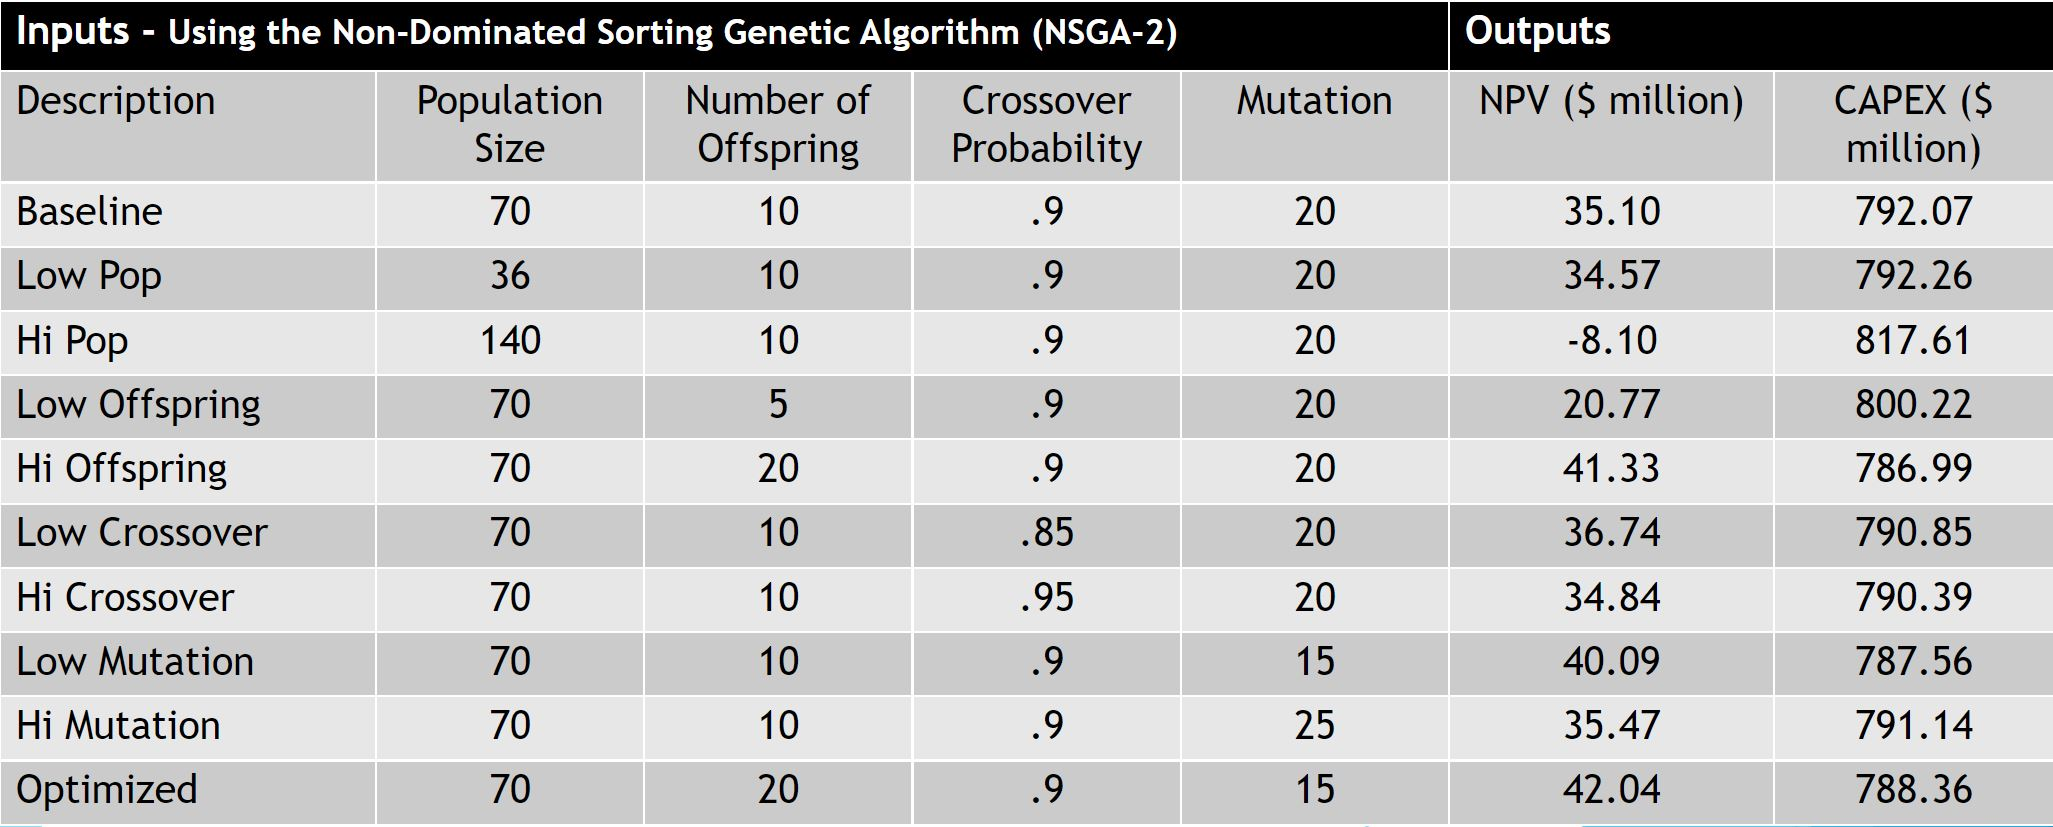
\includegraphics[width=0.7\linewidth]{images/NSGA.jpg}
\caption{Non-Dominated Sorting Genetic Algorithm (NSGA-2) parameter exploration and optimization results}\label{NSGA:1}
\end{figure*}

%%%%%%%%%%%%% end figure %%%%%%%%%%%%%%%%%%%

Next, we looked at the SMS-EMOA algorithm to see how it performed compared to the NSGA-2 and single objective optimization methods. In this case we ran the algorithm with the default parameters, while using the same initial starting design vector as was used with NSGA-2. In this case the SMS-EMOA method found a better MOO optimum than the NSGA-2 method t. It's worth noting, however, that the SMS-EMOA required over 21 times the number of iterations to complete the optimization process. The end result and number of iterations through the optimizer can be seen in Table \ref{EMOA:1}. It's also worth noting that the results of the SMS-EMOA method include very small changes in the design vector fed back into the experimentation module. These steps are extraordinarily small and from a practicality standpoint may be overcome by system noise or other  limitations such as manufacturing quality, sensor limitations, or control system limitations. If factors such as these are not applicable to the given problem, then SMS-EMOA may be a desirable algorithm to use. The number of iterations required to perform this optimization method was 60,051 iterations. This was a staggering 23.5 times the worst-case iterations required for the NSGA-2 algorithm.   

%%%%%%%%%%%%% begin table %%%%%%%%%%%%%%%%%
\begin{table}[btp]
\caption[Table]{SMS EMOA vs. NSGA-2}\label{EMOA:1}
\centering{%
\begin{tabular}{llr}
% \begin{tabular}{!{\hspace*{0.5cm}} >{\raggedright\hangindent=1em} p{3cm} d{3.3} @{\hspace*{1cm}} d{3.3} !{\hspace*{0.5cm}}}
\toprule
Description & NPV (USD) & CAPEX (USD) \\
\midrule
SMS – EMOA & \$42.86M &  \$786.68M \\
NSGA-2 & \$42.04M &  \$788.36M \\
\bottomrule
\end{tabular}
}
\end{table}

%%%%%%%%%%%%% end table %%%%%%%%%%%%%%%%%%%
\section{Final Recommendation}
Focusing on the CAPEX positive side of the results, there are many design options along the Pareto Front (Figure \ref{Final Recommendation}). There are tradeoffs to consider when selecting the optimal solution because the system's efficiency is in tension with the maximum value. Looking at the total efficiency of the system's ability is critical, balancing CO2 injection as well as CO2 generation. Table \ref{Options_Table}, illustrates that for the lower CO2 generated per year from Option 3, there is a decrease in CAPEX of \$12.45 MM. Focusing on CAPEX alone and selecting Option 1 will increase the CO2 generated per year by 73 MMT. Neither is an ideal solution, but Option 2 is a fair compromise that balances the system options. 

More importantly, the optimization model is a valuable tool that can assist with evaluating, prospecting, and planning a commercial-scale CCUS plant. Leveraging this tool will allow businesses to assess commercial agreements, permitting request needs, and contract negotiations. Once that preparation work has been done, the tool can also be used as a communication device between the multiple functions that will plan and execute the building, construction, designing, drilling, and monitoring, by demonstrating how design choices in each of these functions will impact the results. Abstractly, this optimization model is similar to a digital twin of a CCUS plant; it can be utilized to align the stakeholder network towards a common goal. 

%%%%%%%%%%%%% begin figure %%%%%%%%%%%%%%%%%
\begin{figure}
\centering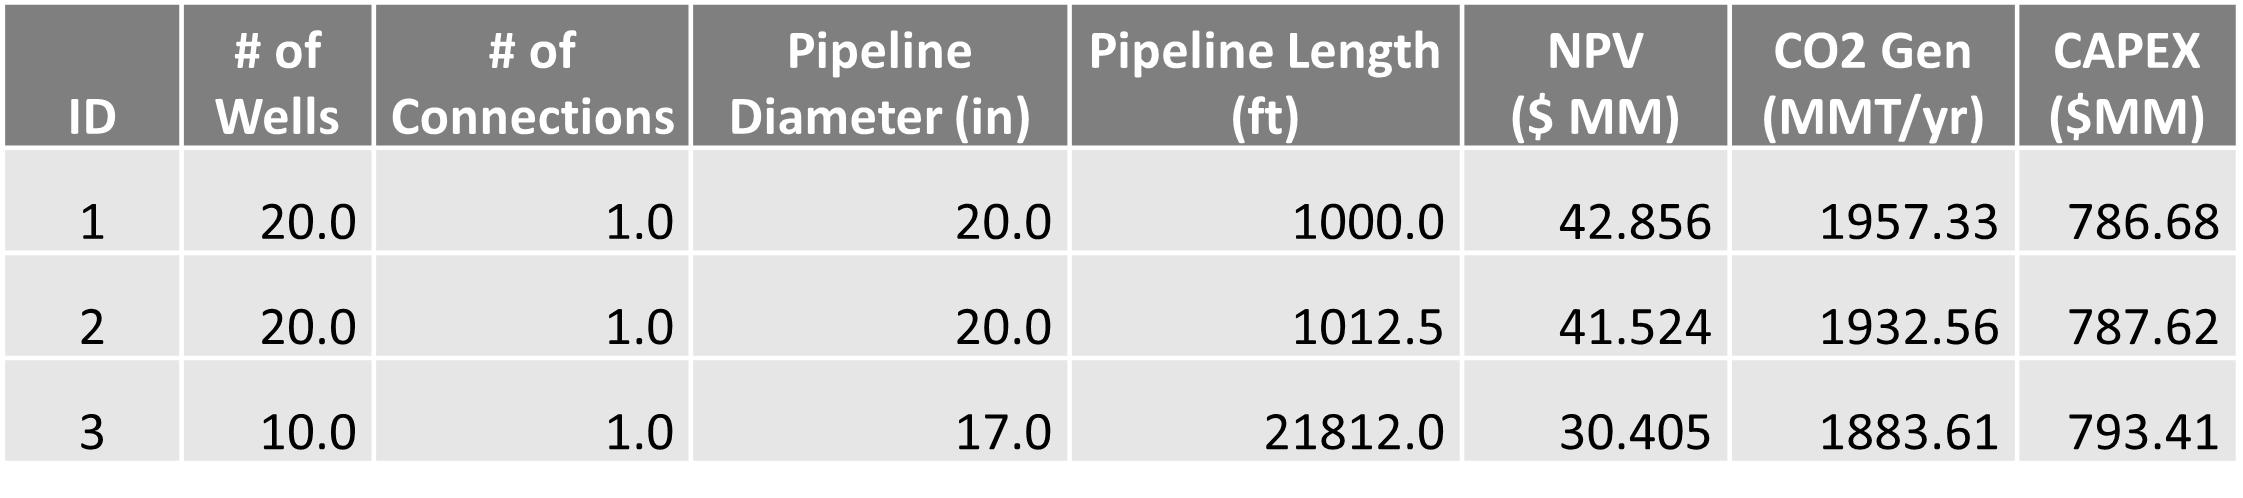
\includegraphics[width=1\linewidth]{images/Options_Table.png}
\caption{Table Recommendation Options}
\label{Options_Table}
\end{figure}
%%%%%%%%%%%%% end figure %%%%%%%%%%%%%%%%%%%

%%%%%%%%%%%%% begin figure %%%%%%%%%%%%%%%%%
\begin{figure}
\centering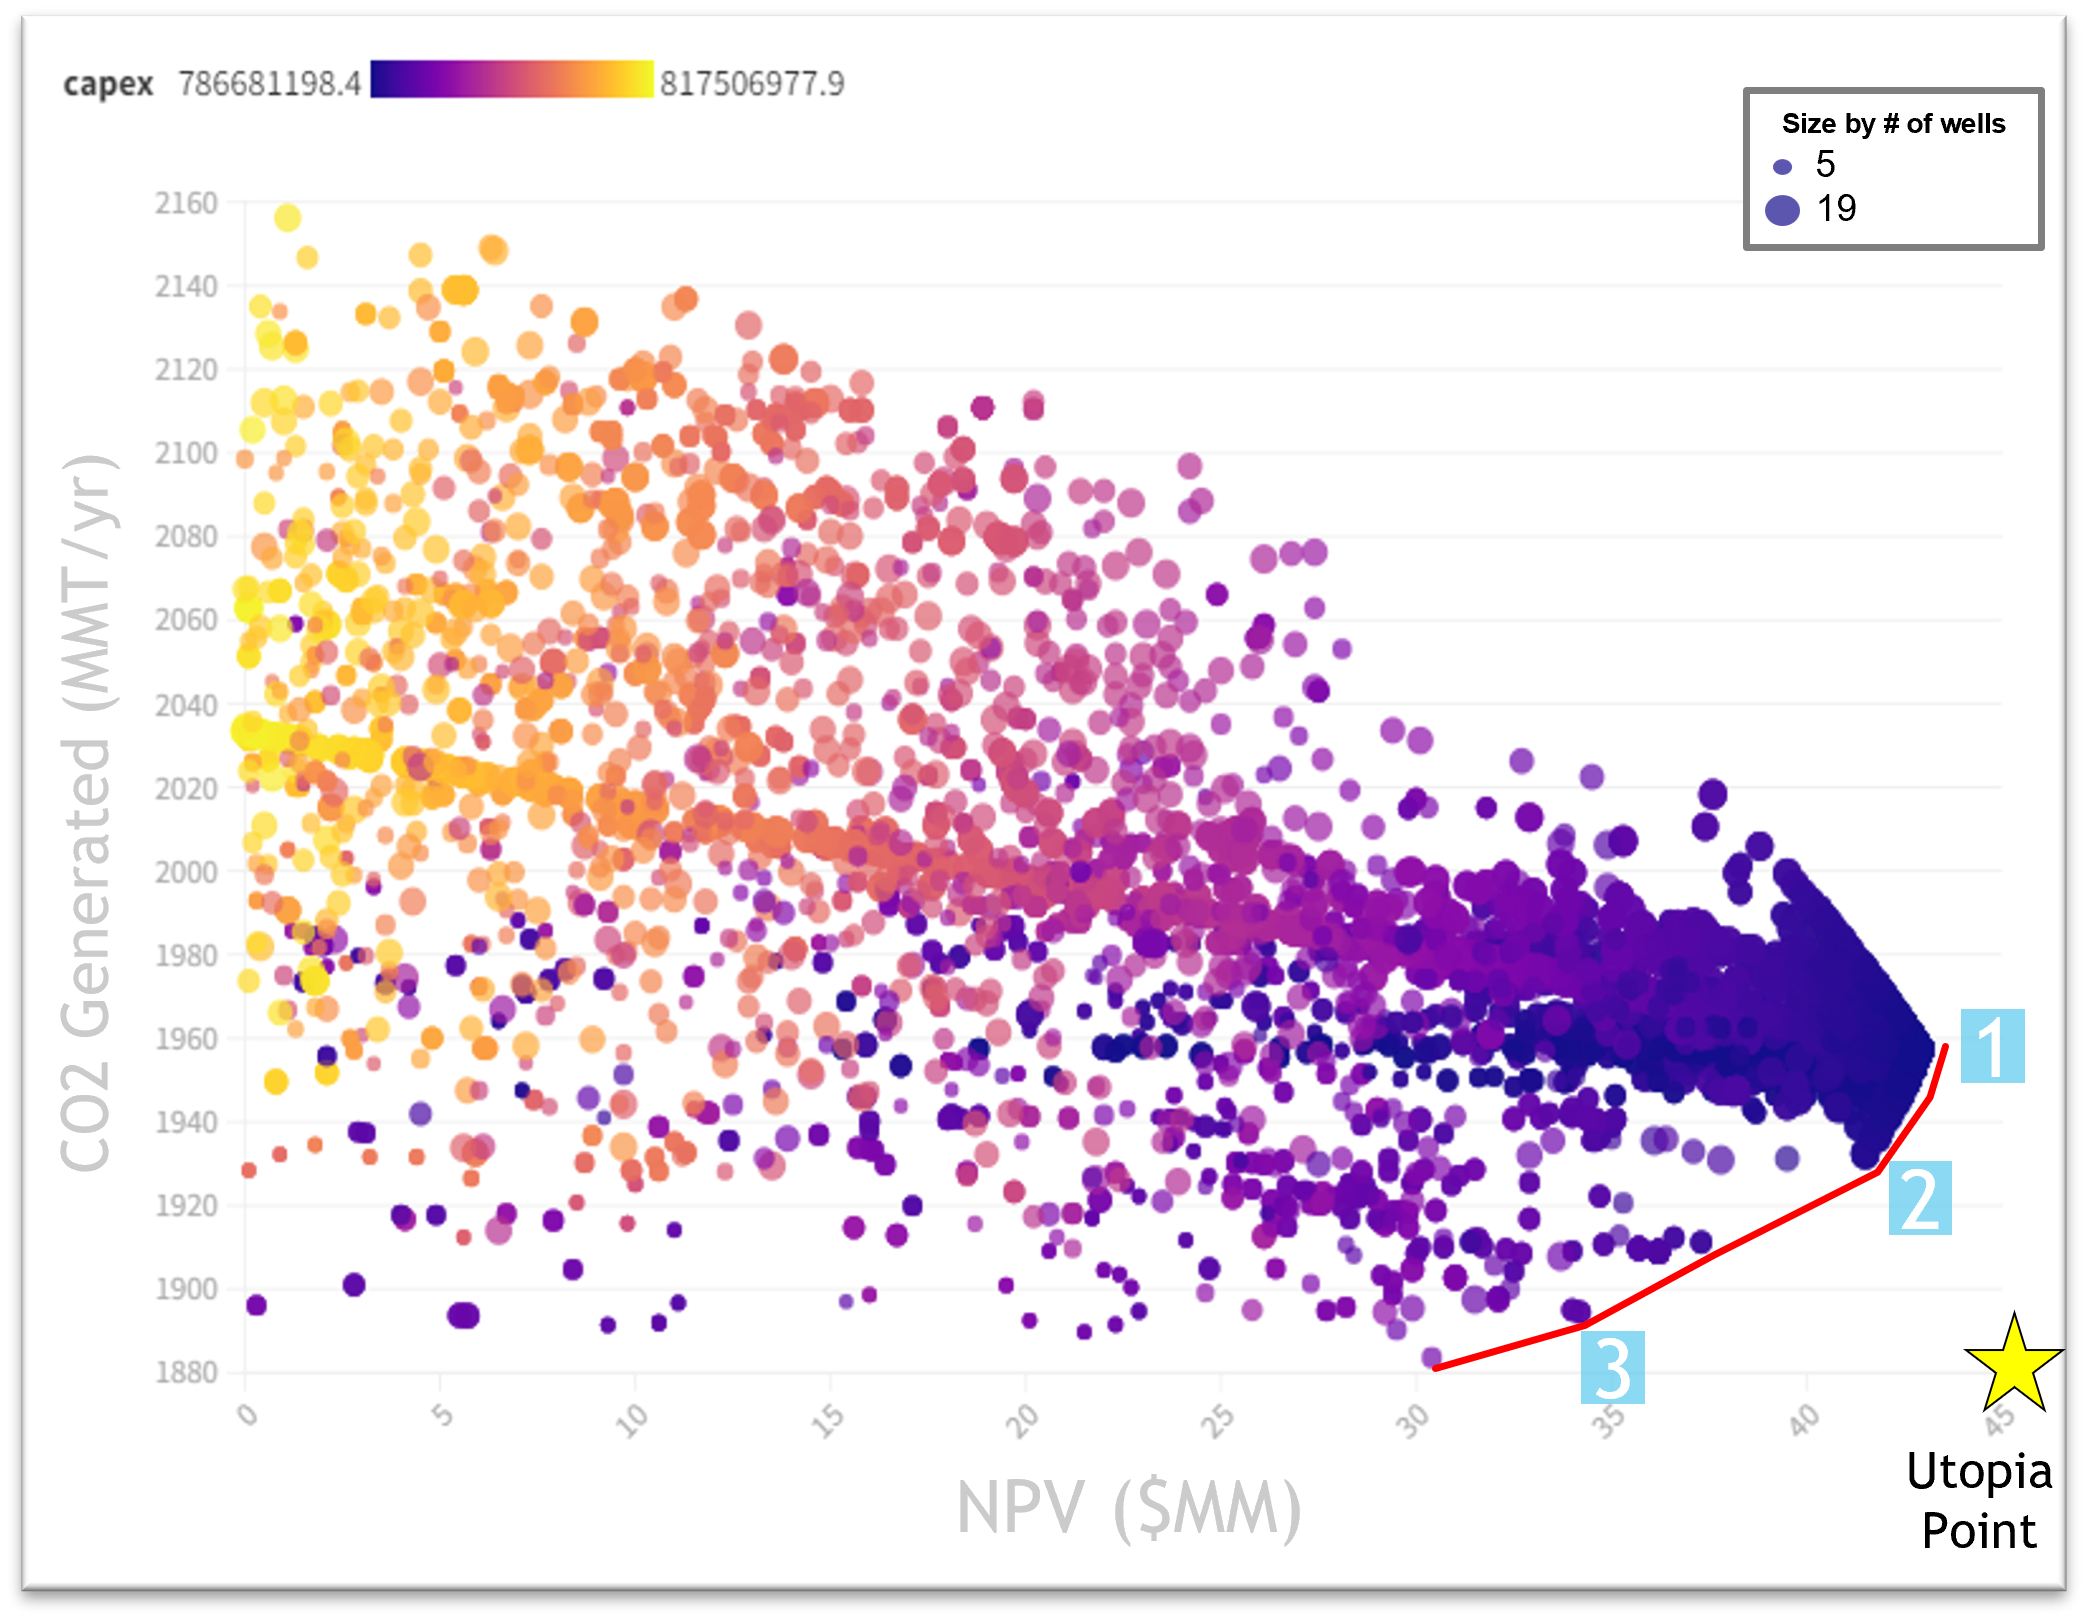
\includegraphics[width=1\linewidth]{images/Final Recommendation.png}
\caption{Final Recommendation Options showing the Pareto Front and Utopia Point}
\label{Final Recommendation}
\end{figure}
%%%%%%%%%%%%% end figure %%%%%%%%%%%%%%%%%%%

\section{Learnings and Future Work}
Reaching the end of this project, the team has greatly enhanced their understanding of multidisciplinary optimization, both from a coding perspective and problem formulation. The following sections summarize the key learnings from the team and future work the group would like to pursue to deepen the value of the project.

\subsection{Learnings}
Working through this project has been an incredible learning opportunity for the team. Not only did it allow us to practice what we were learning in class with a real-world application, but it also gave us a much deeper understanding of the CCUS ecosystem. The project team had varying levels of adjacent experience in this space, but it was generally fairly new to us all.

One key learning we had on the CCUS front was the value of compressing the CO2 at the point-source capture facility before transporting it to the well and injecting it. The first iteration of our model did not have this sequence and instead transported it at ambient conditions and compressed it at the well site. However, once we compressed it before transporting it, we found the supercritical fluid properties (density and viscosity in particular) were much more ideal for transport, and the NPV of the system improved accordingly. Upon additional research, we found that this is the preferred way of transporting CO2 per the literature.

Another important learning for the team was the value of designing for flexibility within the code itself. One team member recommended early on that we create separate files and functions for each module to allow for better collaborative coding and maximum flexibility if we needed to change things throughout the project. When we learned about the supercritical CO2 properties described in the previous paragraph halfway through the semester, this structure in our code made it very simple to switch the sequence of the pipelines and facilities modules within our model. We imagine in real life things like this could come up regularly or there may be a desire to test things like this, and a model architecture that considers this upfront can be very beneficial.

Finally, we found that some optimization methods (i.e. SMS-EMOA) can generate very precise solutions but at very high computational costs.  For some applications these solutions may be so precise that they ultimately be infeasible from an execution standpoint.  As an example, maintaining a system pressure within fractions of a PSI (pounds per square inch) may be infeasible for some systems.

*******************FINAL LEARNING ON OPTIMIZATION METHOD *******************

\subsection{Future Work}
Due to the short time frame of the course, the team had to utilize simplified versions of several modules. As discussed in the problem formulation section, this meant making many upfront assumptions to keep the project scope manageable for a classroom setting. However, if given more time the model could be greatly improved by incorporating these more rigorous techniques.

One such improvement would be to connect our optimizer to a dynamic reservoir simulation model rather than the simplified Darcy's Law equation for the subsurface module. This would allow us to model changes to the pressure in the reservoir as the CO2 is injected and more accurately predict backpressure on the system that would impact injection rates. In reality, we would expect injection rates to decline at some rate over time due to this phenomenon that is currently not accounted for in our system.

The next future improvement would be to model the point-source capture facility distances and CO2 capture rates on a facility-by-facility basis, as opposed to the regional average assumptions we included in this iteration of the model. This would enable us to test each facility discretely in our system to optimize which one(s) we would want to partner with.

Another important future improvement would be to test the incorporation of renewable energy sources into the model to minimize CO2 emissions during compression. The current version of the model indicates that we would emit more CO2 during compression than we would actually store, which defeats the purpose of the system. Some of this may be due to the assumptions made in our facilities module but is certainly worth investigating further with experts regardless.

Finally, expanding some of our bounds for our decision variables could lead to better results. We made the decision to cap the number of wells for this study to twenty to keep CAPEX in a reasonable range. However, it might be useful for the decision-maker to know what the true optimum would be in the system if CAPEX were not a constraint. Another version of the study that greatly expands the number of wells allowed but includes minimizing CAPEX as a third objective could help visualize this tension on the tradespace. It also could enhance the value of tie-ing in multiple facilities, since all of our high NPV results currently only included one facility connection.

We are encouraged by this first multidisciplinary optimization problem and look forward to the opportunity to enhance it further in the future with these and other improvements. Based on the findings, there is much value to be had in a project like this at the current tax incentive rates.


% References section before appendix
\bibliographystyle{asmeconf}  %% .bst file following ASME conference format. Do not change.
\bibliography{asmeconf-sample}%% <=== change this to name of your bib file

\clearpage
\appendix

\section[Appendix A]{Block Diagram}\label{appendix:a}

%%%%%%%%%%%%% begin figure %%%%%%%%%%%%%%%%%
%% captions go below figures
\begin{center}
    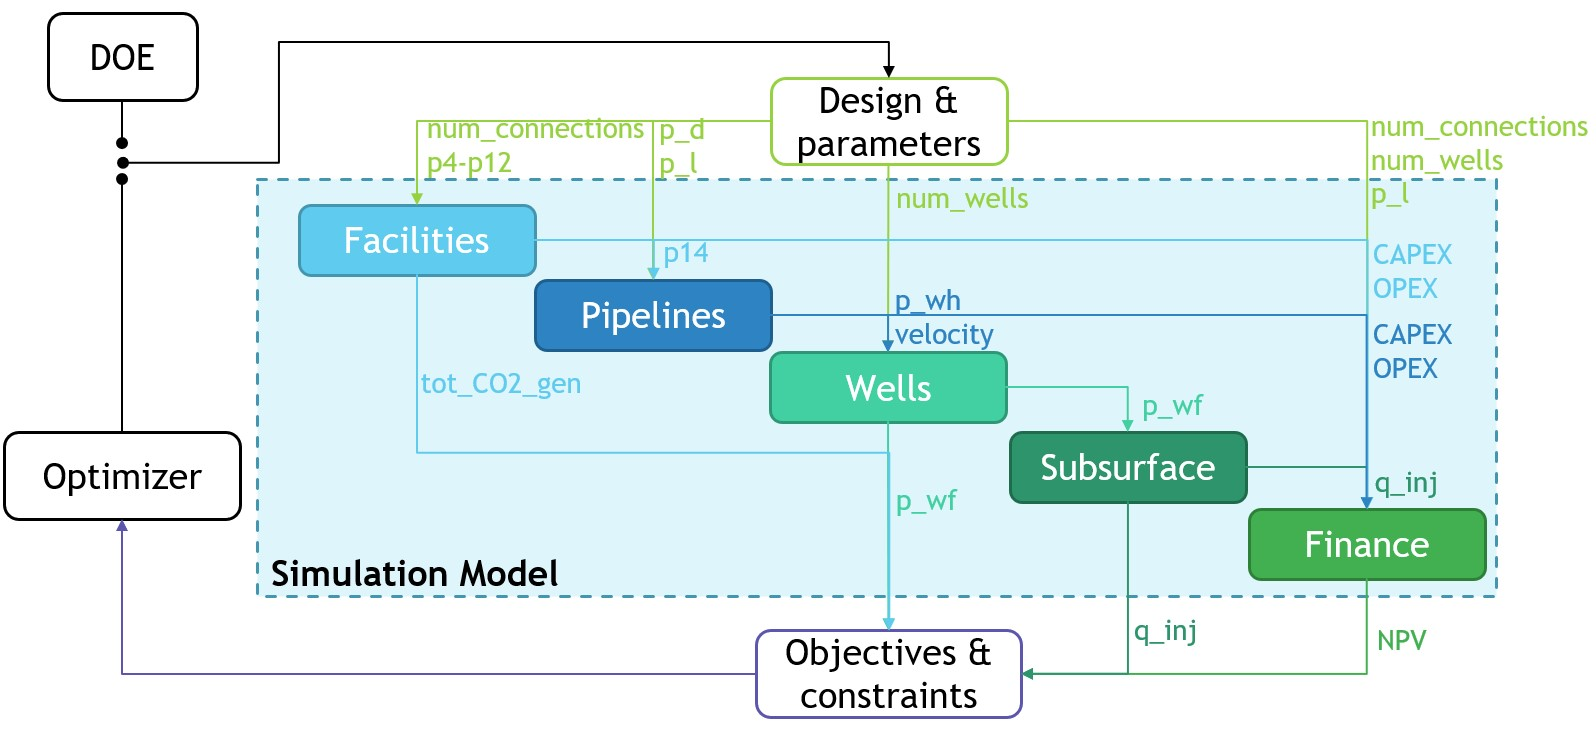
\includegraphics[width=2\linewidth]{images/Block_diagram.jpg}
\end{center}
%\begin{figure*}[H]
%\centering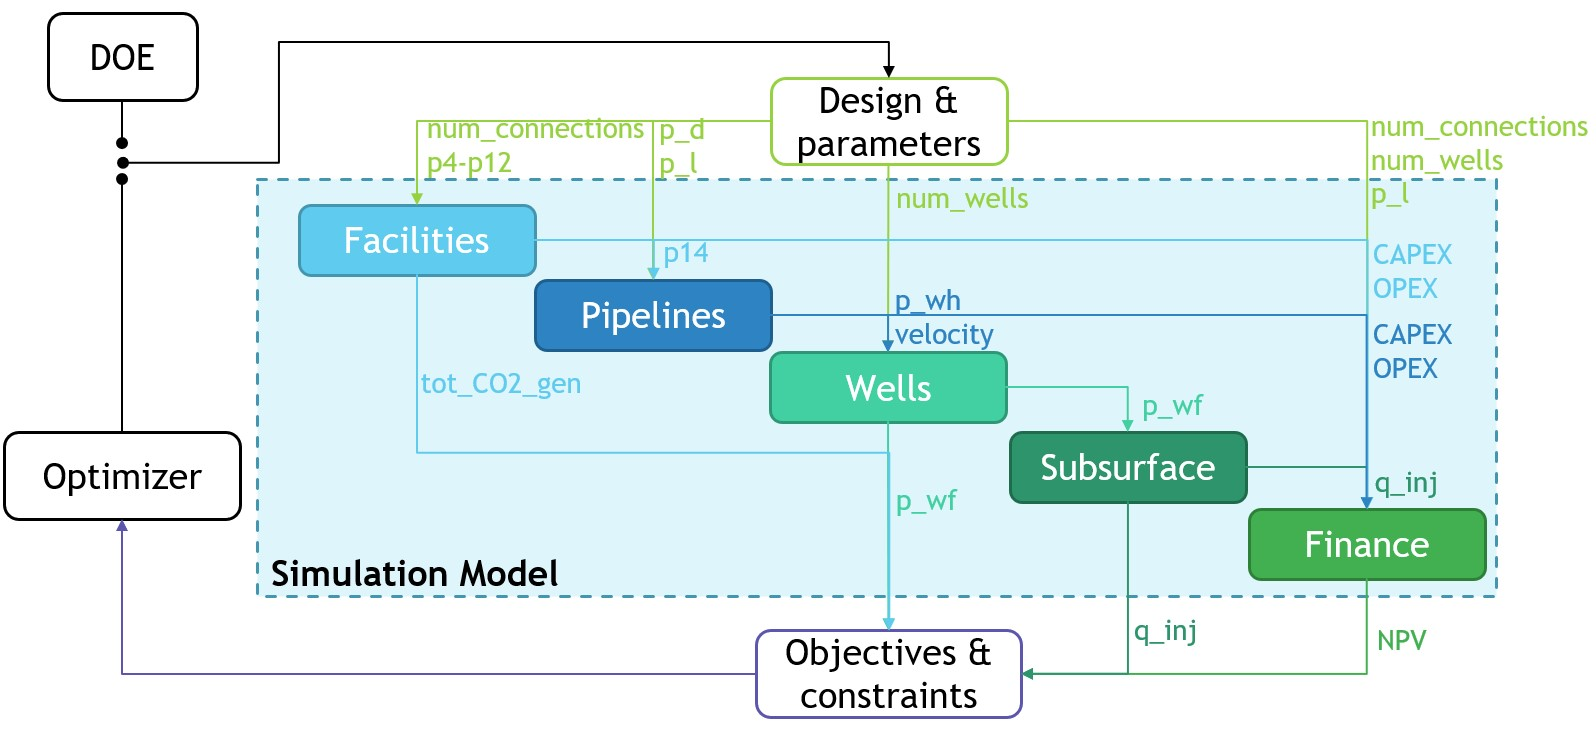
\includegraphics[width=0.7\linewidth]{images/Block_diagram.jpg}
%\caption{System Block diagram}\label{block_diagram:1}
%\end{figure*}
 %%%%%%%%%%%%% end figure %%%%%%%%%%%%%%%%%%%
 \clearpage
\section[Appendix B]{N2 Diagram}\label{appendix:a}
 %%%%%%%%%%%%% begin figure %%%%%%%%%%%%%%%%%
%% captions go below figures
\begin{center}
    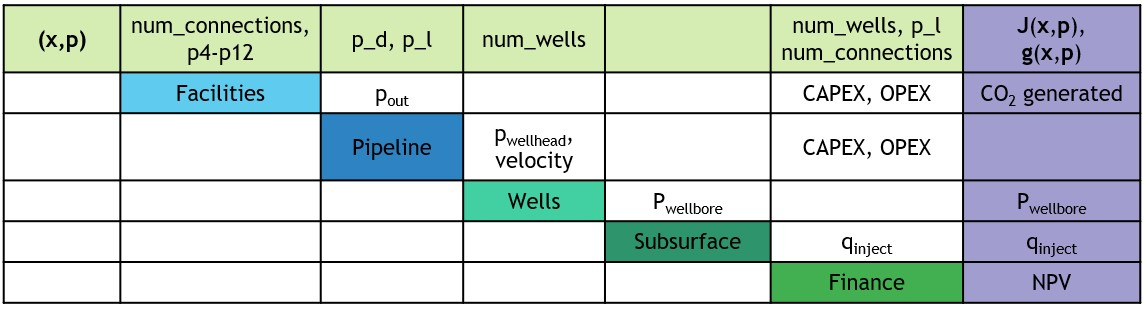
\includegraphics[width=2\linewidth]{images/n2_diagram.jpg}
\end{center}
%\begin{figure*}[h!]
%\centering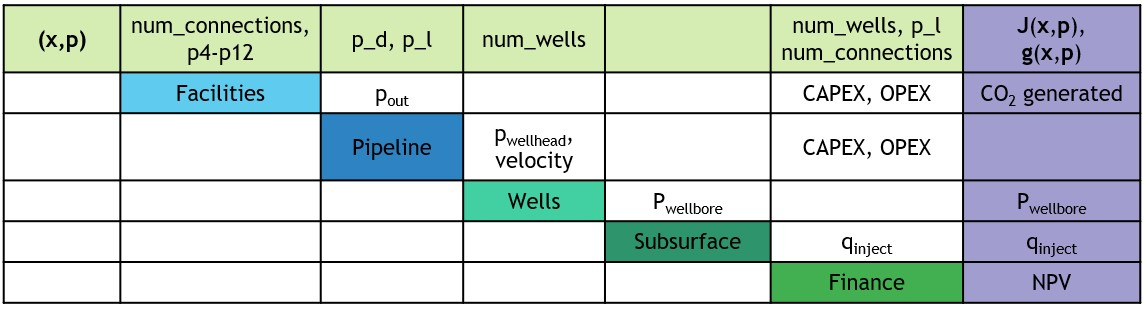
\includegraphics[width=0.95\linewidth]{images/n2_diagram.jpg}
%\caption{N2 diagram}\label{n2_diagram:1}
%\end{figure*}
 %%%%%%%%%%%%% end figure %%%%%%%%%%%%%%%%%%%


%%%%%%%%%  Under here are resources to use to build images and tables %%%%%%%%%%%%%%%%%%%%%%%%%%%%%%%%%


% \section{Introduction}
% The \texttt{\hrefurl{https://ctan.org/pkg/asmeconf}{asmeconf}} class typesets papers with margins, fonts, headings, captions, and reference formats that follow the specifications for conference papers of the American Society of Mechanical Engineers (ASME). In contrast to older ASME \LaTeX\ templates, \texttt{asmeconf} will set internal and external hyperlinks, and the pdf file will contain bookmarks and metadata. Many other useful features have been incorporated. This class is not a publication of ASME, but the author has published in ASME conferences since 1983. 

% The \texttt{.tex} file may be written using standard \LaTeX\ commands, although some specific initial commands are needed to format the blocks containing the author[s], title, and abstract.  This class loads a number of other packages, all of which are contained in up-to-date versions of \hrefurl{https://www.tug.org/texlive/}{\TeX\ Live}, \hrefurl{http://www.tug.org/mactex/}{Mac\TeX}, and similar platforms. If you get an error message about a missing package, you may download it at no cost from CTAN (\hrefurl{https://ctan.org}{ctan.org}). 

% \subsection{Essential Initial Commands}

% To begin, fill in the fields to be completed at top of the \texttt{asmeconf-template.tex} file. These fields include the headers for your conference and your paper number. Specified metadata will be placed into the pdf file itself. 
% The title should be placed into \verb|\title{..}|. 

% Put author names into the \verb|\SetAuthors{name, name,...}| command in the desired order; follow the syntax illustrated \texttt{asmeconf-template.tex} file. Put each distinct address sequentially into a separate \verb|\SetAffiliation{n}{address}|, where $n = 1,2,\ldots$ Tag each author with an affiliation by putting \verb|\affil{n}| after that author's name inside the \verb|\SetAuthors{..| command. 

% Keep author addresses short.  List the author institution, and the City, State (US authors), City, Province, Canada (Canadian authors), or City, Country (other international authors). 

% One author (or more) may be designated as the corresponding author by placing \verb|\CorrespondingAuthor{email}|  after \verb|\affil{n}|. Two or more authors may be joint first authors by putting \verb|\JointFirstAuthor| after \verb|\affil{n}|.

% After setting up the headers, authors,  and title, issue the \verb|\maketitle| command. 

% The abstract text must be placed into \verb|\begin{abstract}| \ldots \verb|\end{abstract}|. The abstract will automatically be italicized. Keywords may be included using the \verb|\keywords{..}| command. The \texttt{keyword} command \textit{must} be issued before the abstract environment. 

% %%%%%%%%%%%%%%%%%%%%%%%%%%%%%%%%%%%%%%%%%%%%%%%%%%%%%%%%%%%

% \section{Referring to Citations, Figures, and Equations}

% Citations are automatically numbered \cite{ning2002}. They should be inserted in the text using a \verb|\cite{ref}| command~\cite{gibson2008,stevens1999}. The citations will be automatically sorted and compressed if they are given in a set \cite{stevens1999,ning2002,gibson2008,wions2005,smith2002,watson1982}. 
% A specific reference may be named with an abbreviation, as in Ref.~\cite{watson1982}.
% See the \texttt{asmeconf-sample.bib} file and Sect.~\ref{sec:references} for examples of entering references.

% For ASME conference papers, the labels Equation and Figure should be abbreviated when they do not start a sentence, as in  Eq.~\eqref{eqn:dw} and Fig.~\ref{fig:1}. Figure~\ref{fig:1} is spelled out when it starts a sentence. Equation~\eqref{eqn:dw} is spelled out when it starts a sentence. 

% Equations are typeset in the usual way and will be automatically numbered.  The class file loads the \texttt{amsmath} and \texttt{mathtools} packages. Further, the \texttt{newtxmath} package used for the math fonts includes many additional features (see Sect.~\ref{sec:moremath}).
% \begin{equation}\label{eqn:fourier}
% \vec{q} = -k\nabla T
% \end{equation}

% ASME prefers SI units. (U.S.\ style units may follow in parentheses.) Be sure to put all symbols into the nomenclature list, including their units.


% %%%%%%%%%%%%% begin figure %%%%%%%%%%%%%%%%%

% %% captions go below figures

% \begin{figure}
% \centering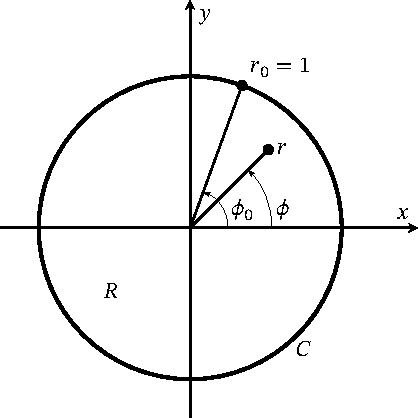
\includegraphics[width=0.7\linewidth]{sample-figure-1.pdf}
% \caption{Caption with math, eqn.~\eqref{eqn:fourier}: $z = (r,\phi)$ \cite{Lienhard2019b}}\label{fig:1}
% \end{figure}
 
% %%%%%%%%%%%%% end figure %%%%%%%%%%%%%%%%%%%


% %%%%%%%%%%%%%%%%%%%%%%%%%%%%%%%%%%%%%%%%%%%%%%%%%%%%%%%%%%%

% %% Use title case for subsections and subsubsections (first letter of words capitalized)

% \section{Section Headings and Captions}

% ASME requires that section headings and captions be set in an uppercase, sans serif font.  The class will do this automatically.  You can place \verb|\cite{..}|, \verb|\ref{..}|, \verb|\label{..}|, and mathematics into headings and captions directly, as you would in the main text. Do not enclose them braces, e.g.\ \verb|{\cite{..}}|, which will cause errors. You can place \verb|\footnote{..}| into headings, but not into captions.\footnote{See \texttt{tex-stackexchange} for various approaches to footnotes in captions, if they seem necessary. For footnotes in tables, use the \texttt{tablefootnote} package.}\footnote{Sequential footnotes are automatically separated by a comma.}

% Text in section headings and captions will not be capitalized if enclosed in a \verb|\NoCaseChange{..}| command.

% Sections may either be numbered or left unnumbered.

% Simple mathematical expressions can be used in either captions or section headings. For a section heading that includes more complicated math (and macros), you may use the optional argument of \verb|\section[..]{..}| to create a pdf bookmark without losing characters or producing warnings or errors. See the \texttt{asmeconf-template.tex} source file for examples of this procedure. These bookmarks should usually be text expressions, although some math is supported.  

% To override the \texttt{sansbold} math version in captions, put \verb|\NoCaseChange{\mathversion{normal}}| in the caption.

% \subsection{Subsection and Sub-subsection Headings}

% Subsections and sub-subsection headings should be entered in title case, with the first letter of primary words capitalized. Sub-subsections (i.e., paragraphs) are never numbered.


% %%%%%%%%%%%%%%% begin simple table %%%%%%%%%%%%%%%%%%%%%%%%%% 

% %% Captions go above tables
% %%
% %% Note that placement of figures and tables can managed with the [!tbhp] options. See: https://latexref.xyz/dev/latex2e.html#Floats

% \begin{table}[t]
% \caption[Table]{A simple table}\label{tab:1}
% \centering{%
% \begin{tabular}{llr}
% \toprule
% Experiment & $u$ [m/s] & $T$ [\textdegree C] \\
% \midrule
% Run 11 & 12.5 & 103.4 \\
% Run 12 & 24   & 68.3 \\
% \bottomrule
% \end{tabular}
% }
% \end{table}

% %%%%%%%%%%%%%%%% end table  %%%%%%%%%%%%%%%%%%%%%%%%%%%%%%%%%%%% 

% %%%%%%%%%%%%%%% begin more complicated table %%%%%%%%%%%%%%%%%%%%%%%%%%%%%%%%%%%%

% \begin{table}[t]
% \caption{Table with more complicated columns}\label{tab:2}%
% \centering{%
% \begin{tabular}{!{\hspace*{0.5cm}} >{\raggedright\hangindent=1em} p{3cm} d{3.3} @{\hspace*{1cm}} d{3.3} !{\hspace*{0.5cm}}}
% \toprule
% Experiment & \multicolumn{1}{c@{\hspace*{1cm}}}{$u$ [m/s]} & \multicolumn{1}{c!{\hspace*{0.5cm}}}{$T$ [\textdegree C]} \\
% \midrule
% The first test we ran this morning   & 124.3     &   68.3   \\
% The second test we ran this morning  &  82.50    &  103.46  \\
% Our competitor's test                &  72.321   &  141.384 \\
% \bottomrule
% \end{tabular}
% }
% \end{table}

% %%%%%%%%%%%%%%%% end table  %%%%%%%%%%%%%%%%%%%%%%%%%%%%%%%%%%%% 

% %%%%%%%%%%%%%%% begin two column table %%%%%%%%%%%%%%%%%% 
% \begin{table*}
% \caption{A table spanning two columns}\label{tab:3}%
% \centering{%
% \begin{tabular*}{0.8\textwidth}{@{\hspace*{1.5em}}@{\extracolsep{\fill}}ccc!{\hspace*{3.em}}ccc@{\hspace*{1.5em}}}
% \toprule
% \multicolumn{1}{@{\hspace*{1.5em}}c}{$x$\rule{0pt}{11pt}} &
% \multicolumn{1}{c}{$\textrm{erf}(x)$} &
% \multicolumn{1}{c!{\hspace*{3.em}}}{$\textrm{erfc}(x)$} &
% \multicolumn{1}{c}{$x$} &
% \multicolumn{1}{c}{$\textrm{erf}(x)$} &
% \multicolumn{1}{c@{\hspace*{1.5em}}}{$\textrm{erfc}(x)$} \\ \midrule
% 0.00 & 0.00000 & 1.00000 & 1.10 & 0.88021 & 0.11980\rule{0pt}{11pt} \\
% 0.05 & 0.05637 & 0.94363 & 1.20 & 0.91031 & 0.08969 \\
% 0.10 & 0.11246 & 0.88754 & 1.30 & 0.93401 & 0.06599 \\
% 0.15 & 0.16800 & 0.83200 & 1.40 & 0.95229 & 0.04771 \\
% 0.20 & 0.22270 & 0.77730 & 1.50 & 0.96611 & 0.03389 \\
% 0.30 & 0.32863 & 0.67137 & 1.60 & 0.97635 & 0.02365 \\
% 0.40 & 0.42839 & 0.57161 & 1.70 & 0.98379 & 0.01621 \\
% 0.50 & 0.52050 & 0.47950 & 1.80 & 0.98909 & 0.01091 \\
% 0.60 & 0.60386 & 0.39614 & 1.82\makebox[0pt][l]{14} & 0.99000 & 0.01000 \\
% 0.70 & 0.67780 & 0.32220 & 1.90 & 0.99279 & 0.00721 \\
% 0.80 & 0.74210 & 0.25790 & 2.00 & 0.99532 & 0.00468 \\
% 0.90 & 0.79691 & 0.20309 & 2.50 & 0.99959 & 0.00041 \\
% 1.00 & 0.84270 & 0.15730 & 3.00 & 0.99998 & 0.00002 \\[2pt]
% \bottomrule\end{tabular*}
% }
% \end{table*}

% %%%%%%%%%%%%%%%%% end two column table  %%%%%%%%%%%%%%%%%%%%%%%%%%%%%%% 

% %%%%%%%%%%%%%%%%%%%%%%%%%%%%%%%%%%%%%%%
% \section{Tables and Figures}

% Table \ref{tab:1} is an example of a simple table. Table captions should be placed above tables.
% The class loads the \texttt{booktabs} package (used for horizontal rules in Tables \ref{tab:1} and \ref{tab:2}), and the \texttt{array} and \texttt{dcolumn} packages which provide extended capabilities for columns in the \texttt{tabular} environment (see Table \ref{tab:2}).  Table \ref{tab:3} is an example of a table that spans two columns. Two column tables (and figures) will always float to the top of a later page.

% Figure captions go below figures. Figure~\ref{fig:2} is an example of a figure that spans two columns and includes subfigures. The text in figures (and tables) should be no smaller than 6~point type. Images in figures are handled by the standard \texttt{graphicx} package.

% Landscape figures and tables may be produced at full-page size by putting \verb|\usepackage[figuresright]{rotating}| in your \texttt{.tex} file's preamble and using the \texttt{sidewaystable*} and \texttt{sidewaysfigure*} environments~\cite{fairbairns}.


% %%%%%%%%%%%%%%%%%%%%%%%%%%%%%%%%%%%%%%%%%%%%%%%%%%%%%%%%%%%%%%%%%%%%%%

%\section{Reference Formatting with \NoCaseChange{\texttt{asmeconf.bst}}\footnote{To prevent capitalization of text in a section heading or caption, such as an SI unit, enclose it in a \texttt{\textbackslash NoCaseChange} command. As of the July 2022 release of \LaTeX, commands used in a heading or caption may be protected globally by putting this in the preamble: \texttt{\textbackslash AddToNoCaseChangeList\{\textbackslash MyCommand\}}.}}\label{sec:references}

% The {\upshape\texttt{asmeconf.bst}} \hologo{BibTeX}  style follows the reference styles shown on ASME's conference web site in  2022.\footnote{\texttt{asmeconf.bst} is intended as a replacement for the old \texttt{asmems4.bst}, which does not follow ASME's current reference formats or support DOI and URL.}
% Examples for these and many other cases are given in the \texttt{asmeconf-sample.bib} file, which is part of this distribution. Citations and references are managed by the standard \texttt{natbib} package.  Nevertheless, a few comments are necessary. 

% %% sub-subsections should *not* be numbered according to ASME's style

% \subsubsection*{DOI, URL, and eprint} Include DOI numbers when they are available.  URL's may alternatively be given. ASME requests that URLs point to a document's abstract.

% Basic support for \texttt{eprint} numbers is also included, generating a url at the end of the citation. The \texttt{archive} type may be specified using the macros \texttt{arxiv, google\-books, hdl, jstore, oclc}, or \texttt{pubmed} (e.g., \texttt{archive=hdl},  \textit{without} braces). Both \texttt{eprint} and \texttt{archive} fields \textit{must} be given. Other root urls may be invoked using \verb|archive = {https://another.url.org/}|.

% \subsubsection*{Online Sources} A bibliography entry \verb|@online{..| is included for citation of online sources, such as web pages. A \texttt{url} or \texttt{eprint} with \texttt{archive} must be included. See the examples of use in the \texttt{asmeconf-sample.bib} file. 

% \subsubsection*{Date Accessed} The \verb|urldate={..}| field may be used to provide the date on which a given url was accessed. By default, the text printed will be \texttt{Accessed `date',}. The word ``Accessed'' may be changed using the \verb|urltype={..}| field.

% \subsubsection*{Conference Location and Date} To specify the city and date of a conference, you can use \verb|venue={..}| and \verb|eventdate={..}| with the entries \verb|@inproceeedings{..| and \verb|@proceeedings{..|.

% \subsubsection*{Capitalization of Titles} ASME's bibliography style requires that document titles be in title case. The first letters of principal words are capitalized. Do this in the \texttt{.bib} file.



% %%%%%%%%%%%%%%%%%  begin two column figure  %%%%%%%%%%%%%%%%%%%%%%%%%%%

% \begin{figure*}
% \begin{subfigure}[t]{0.5\textwidth} % subfigure is basically the same as minipage
% \vbox{
% \vspace*{1.7em}
% \centering{
%   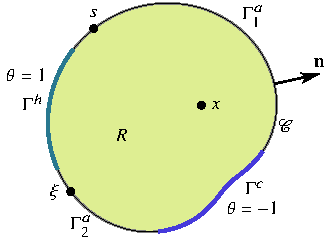
\includegraphics{sample-figure-2a.pdf}
% }%
% \vspace*{1.7em}
% }%
% \subcaption{Interior region\label{fig:interior-region}}
% \end{subfigure}%
% %%%%%%%%%%%%% no spaces or line breaks between these two subfigures
% \begin{subfigure}[t]{0.5\textwidth}
% \centering{%
% 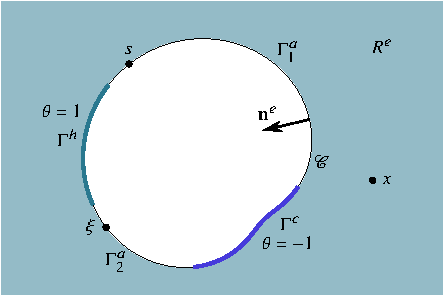
\includegraphics{sample-figure-2b.pdf}
% }%
% \subcaption{Exterior region\label{fig:exterior-region}}
% \end{subfigure}
% \caption{A figure with two subfigures  \cite{lienhard2023}\label{fig:2}}
% \end{figure*}

% %%%%%%%%%%%%%%%%%%%  end two column figure  %%%%%%%%%%%%%%%%%%%%%%%%%%


% %%%%%%%%%%%%%%%  MORE ON MATH   %%%%%%%%%%%%%%%%%%%%%%%%%%%%%%%%%%%%%%%%%%%%%%%%%%%%%%%%%%%%%%%%%%%%%%

% %% Here is an example of managing complicated math in a section or subsection heading: 
% %%    the optional argument to \section will provide the pdf bookmark
% %%    without losing characters or producing warnings/errors.
% %%
% %% In this heading, letter u is forced to be upright with \mathrm{u}
% %%
% \section[More on math: u\cdot\omega=0]{More on math: $\vec{\mathrm{u}}\cdot\vec{\omega}=0$}\label{sec:moremath}

% In most cases, the need for a wide equation can be eliminated by using one of the multiline equation environments defined by 
% \texttt{amsmath}, such as \texttt{align}, \texttt{split}, or \texttt{multline}~\cite{amsmath}. The following equation is set with the 
% \texttt{multline} environment:
% \begin{multline}\label{eqn:energy}
% \frac{\partial}{\partial t}\left[\rho\bigl(e + \lvert\vec{u}\rvert^2\big/2\bigr)\right]  + \nabla\cdot\left[\rho\bigl(h + \lvert\vec{u}\rvert^2\big/2 \bigr)\vec{u}\right] \\
%  ={}-\nabla \cdot \vec{q} +  \rho \vec{u}\cdot\vec{g}+ \frac{\partial}{\partial x_j}\bigl(d_{ji}u_i\bigr) + \dot{Q}_v
% \end{multline}
% An example using \texttt{align} appears in Appendix~\ref{appendix:a}.

% An alternative solution may be to set large equations into two-column-wide tables or figures. An experimental package for setting equations that span two columns, \texttt{asmewide.sty}, can be loaded as well, but that code may require hand-fitting around figures, tables, and page breaks. See the examples in~\cite{lienhard2022}.

% Math italics are used for Roman and Greek letters by default.  If you want an upright letter in math, you can use the relevant math alphabet, e.g., \verb|\mathrm, \mathbf, \mathsf|:
% \begin{equation}\label{eqn:dw}
% \vec{F} = m \vec{a} \quad\textrm{or}\quad \vec{\mathrm{F}} = m \vec{\mathrm{a}} \quad\textrm{or}\quad \mathbf{F} = m \mathbf{a} \quad\textrm{or}\quad \vec{\mathsf{F}} = m \vec{\mathsf{a}}
% \end{equation}
% To get additional symbols in bold math, use the \verb|\bm{..}| macro from the \texttt{bm} package (which is loaded by the class) or, for longer passages, use \verb|{\mathversion{bold}|\ldots\texttt{\}}.

% The class file also provides upright sans-serif Greek letters with \verb|\sfalpha| and similar expressions (e.g., $\sfalpha, \sfbeta, \sfgamma, \sfdelta$ \ldots $\bm{\sfalpha, \sfbeta, \sfgamma, \sfdelta \ldots}$), in case they are needed (but note that the \verb|newtxmath| options \verb|frenchmath| and \verb|slantedGreek| also affect how Greek letters are presented).

% \subsection{The \texttt{newtxmath} and \texttt{mathalpha} Packages~\cite{sharpe1,sharpe2}} The \texttt{newtxmath} package~\cite{sharpe1}, loaded by default, includes many options for mathematics, most of which can be called as options to \verb|\documentclass|. For example, the \texttt{upint} option selects upright integral signs (rather than slanted integral signs):
% \begin{quote}
% \verb|\documentclass[upint]{asmeconf}|. 
% \end{quote}  
% The option \verb|subscriptcorrection| improves the spacing of math subscripts. These math options are discussed further in the \texttt{asmeconf-template.tex} file. 

% In addition, many options for calligraphic, fraktur, and script fonts are available as options to the \texttt{mathalfa} package, which is also loaded. These may be invoked, for example, as 
% \begin{center}
% \verb|\documentclass[mathalfa=cal=boondoxo]{asmeconf}| 
% \end{center}
% which selects a Boondox font for \verb|\mathcal|, as in $A \in \mathcal{P}(A)$. To find all the font options, refer to the \texttt{mathalfa} package documentation \cite{sharpe2}.

% The \texttt{asmeconf} class is designed to be used with \texttt{newtxmath} and does not support the \texttt{unicode-math} package.


% %%%%%%%%%%%%%%%  ADDITIONAL PACKAGE OPTIONS  %%%%%%%%%%%%%%%%%%%%%%%%%%%%%%%%%%%%%%%%%%%%%%%%%%%%%%

% \section{Additional Options for \NoCaseChange{\texttt{asmeconf.cls}}}
% The class accepts a number of options in addition to those already described. These options are discussed next.

% \subsection{Colored Hyperlinks}
% ASME requires that all text be \textbf{in black} when the paper is submitted for publication.  For other uses, authors may
% obtain colored hyperlinks with the [\texttt{colorlinks}] option.

% \subsection{Final Column Balancing} The option \texttt{[balance]} invokes the the \texttt{flushend} package~\cite{tolusis}.
% This package will attempt to give equal height to the two columns on the last page. The performance of this package is sometimes inconsistent (with odd page layout or, very rarely, errors), so use this option with caution.

% \subsection{Line Numbers} The option \texttt{[lineno]} invokes the the \texttt{lineno} package~\cite{bottcher}. This option will produce line numbers in the margins. You must run \LaTeX\ \textit{twice} for proper placement of the numbers. Tables, captions, and footnotes will not be numbered.  Line numbers can be helpful for review and editing, but should not be used in your final manuscript. See the documentation of the \texttt{lineno} package for further commands to control line numbering. 

% The \texttt{lineno} package is not compatible with the \texttt{flushend} package that makes final short columns the same height. Balancing is automatically disabled when this option is called. 

% \subsection{Grid-Style Author Block} The option \texttt{[grid]} invokes ASME's grid-style arrangement of author names. Author names are recognized by the commas that separate them. (To include a comma in a name, enclose the name in braces.) Line breaks (\verb|\\|) may be inserted into the address of \verb|\SetAffiliation{n}{address}| as needed. 

% Note that ASME interprets the author order in the grid style by reading names from left-to-right in the top row, then left-to-right in each subsequent row.

% \subsection{Changing the Copyright Footer} The option \texttt{[nofoot]} will omit the ASME copyright from the page footer. The option \texttt{[govt]} will produce a copyright notice for authors who are employees of the U.\ S.\ Government.  The option \texttt{[contractor]} will produce a copyright
% notice for authors who are employed by a U.\ S.\ Government contractor.

% The footers are generated with the \texttt{fancyhdr} package~\cite{oostrum} and can be changed using the commands of that package. Only the default arrangement matches ASME's style, however.

% \subsection{Archivability:~PDF/A} Compliance with PDF/A standards can be enabled using the option \texttt{[pdf-a]} 
% when running with \hologo{pdfLaTeX}. The default setting is for PDF/A-3u with sRGB OutputIntent (\texttt{sRGB.icc}). 
% If levels 1b, 2b, 2u, or 3b are preferred, use the options \texttt{[pdfapart=1 or 2 or 3]} and 
% \texttt{[pdfaconformance=b or u]}. Note that accessible conformance~(\texttt{a}) is not currently possible with \LaTeX.

% As of late 2021, the \LaTeX 3 team is phasing in native support for PDF/A in the \LaTeX\ kernel, which will make these
% class options unnecessary when using up-to-date installations.

% \subsection{Superiors Font} The \texttt{newtxtext} package includes a superiors font (both numbers and letters) for use in footnote markers and text superscripts. To enable this font, use the option \texttt{[nodefaultsups]}. 

% \subsection{Typewriter Font Options} This font is the sans-serif \texttt{inconsolata}. By default, the word spacing is variable, but option \texttt{[mono]} ends this behavior. A slashed zero is the default; option \texttt{[var0]} removes the slash. Option \texttt{[hyphenate]} enables hyphenation. (The hyphenation option is not available if the \texttt{[fontspec]} option is used.)

% \subsection{Support for Other Languages}  This package can be adapted to incorporate (or entirely use) languages other than English. See Appendix \ref{appendix:b} for details.


% %%%%% Conclusions %%%%%%%%%%%%%%%%%%%%%%%%%%%%%%%

% \section{Conclusion}
% Provide a brief conclusion (3-4 lines).


% %%%%% Acknowledgments %%%%%%%%%%%%%%%%%%%%%%%%%%%

% \section*{Acknowledgments}
% Place any acknowledgments here.


% %%%  REFERENCES  %%%%%%%%%%%%%%%%%%%%%%%%%%%%%%%%
% %%
% %% Put your references into your .bib file in the usual way. Run latex once, bibtex once, then latex twice.
% %% The asmeconf.bst style allows @inproceedings and @proceedings to include: 
% %%		venue = {Location of Conference}, 
% %%		eventdate = {Month, days},

% \nocite{*}%% <=== Delete this line unless you want to typeset the entire contents of your .bib file!

%\bibliographystyle{asmeconf}  %% .bst file following ASME conference format. Do not change.
%\bibliography{asmeconf-sample}%% <=== change this to name of your bib file


% %%%  APPENDICES  %%%%%%%%%%%%%%%%%%%%%%%%%%%%%%%%
% \appendix

% %% Note that appendices will be "numbered" A, B, C, ... etc. Use \section, not \section*
% %% Equations will be numbered sequentially following those in the paper. Do not reset the equation counter.

% %% Here we use the optional argument to control the pdf bookmark and prevent errors.
% \section[The Vector Product A\times B]{The vector product $\vec{A}\times\vec{B}$}\label{appendix:a}

% This brief illustration of an appendix shows the numbering of the appendix and equations. Equations are numbered
% consecutively, following those in the paper. Consider $\rho \neq \textrm{fn}(p)$:
% \begin{align}
% \frac{d\Gamma}{dt} &{}= \frac{d}{dt} \int_{\mathcal{C}} \mathbf{u} \cdot d\mathbf{r}\\
% 				   &{}= \int_{\mathcal{C}} \frac{D\mathbf{u}}{Dt} \cdot d\mathbf{r} + \underbrace{\int_{\mathcal{C}} \mathbf{u}\cdot d\biggl( \frac{d\mathbf{r}}{dt}\Biggr)}_{=\, 0} \\[-2pt]
%                    &{}= \iint_{\mathcal{S}} \nabla \times \frac{D\mathbf{u}}{Dt}  \cdot d\mathbf{A}\\
%                    &{}= \iint_{\mathcal{S}}  \nabla p \times \nabla \left( \frac{1}{\rho}\right) \cdot d\mathbf{A}
% \end{align}

% %%%%%%%%%%%%%%%%%%%%%%%%%%%%%%%%%%%%%%%%%%%%%%%%%%%%%%%%%%%%%%%%%%%%%%
% \section{Multilingual Support}\label{appendix:b}

% ASME publishes in English, but the \texttt{babel} package is loaded for 
% users who may wish to include other languages. For example, an author might wish to include an appendix that provides the 
% abstract in another language.

% When more than one language option is included in \verb|\documentclass[..]{asmeconf}|, English will be 
% assumed to be the main language of the document. (To choose a different main language, set \texttt{[main=..]}).
% If no language options are given, the package defaults to English.  As examples, a passage in French is 
% shown in \selectlanguage{french}\appendixname~\ref{app:fourier}\selectlanguage{english}, followed by 
% \ifpdftex abstracts in Spanish, Greek, Russian, and Vietnamese.\else abstracts in other languages.\fi

% The input encoding can be utf-8, as for these glyphs:
% %% If you have trouble with the next line, your file may not be saved in utf-8 format. You can delete that line to resolve the issue.
% \typeout{If you have trouble with the next line, your file may not be saved in utf-8 format. You can delete that line to resolve the issue. Under LuaLaTeX, you can load the [fontspec] option if you have the relevant systems fonts installed}%
% àáâäæãåā  èéęëêēė  îïíīįì ôöòóœøōõ ûüùúū çćč ł ñń ßśš ÿ žźż.

% Fonts similar to Times/Helvetica are automatically used when the Greek, Vietnamese, or selected cyrillic-alphabet languages are called as options under {\upshape\hologo{pdfLaTeX}}. Using {\upshape\hologo{LuaLaTeX}} with the \texttt{[fontspec]} option, many additional scripts are available; see the supplemental notes for such usage~\cite{lienhard2021}. Possibilities include Arabic, Bengali, Chinese, Devanagari (e.g., for Hindi), Hangul (for Korean), Kana (for Japanese), and Tamil. \textit{The {\upshape\texttt{[fontspec]}} option requires a \LaTeX\ installation dated October 2020 or later.}

% The bibliography style, \texttt{asmeconf.bst}, is designed in English and aimed at \hologo{BibTeX}.  
% % Multilingual bibliographies can be supported using \texttt{BibLaTeX}.

% %%%%%%%%%%%%%%%%%%%%%%%%%%%%%%%%%%%%%%%%%%%%%%%%%%%%%%%%%%%%%%%%%%%%%%

% \begin{selectlanguage}{french}%
% \section{Discours Préliminaire de Fourier}\label{app:fourier}
% Les causes primordiales ne nous sont point con­nues; mais elles sont assujetties à des lois simples et constantes, que l'on peut découvrir par l'obser­vation, et dont l'étude est l'objet de la philosophie naturelle. 

% La chale ur pénètre, comme la gravité, toutes les substances de l'univers, ses rayons occupent toutes les parties de l'espace. Le but de notre ouvrage est d'exposer les lois mathématiques que suit cet élé­ment. Cette théorie formera désormais une des branches les plus importantes de la physique gé­nérale~\cite{fourier1822}. 
% \end{selectlanguage}%
 
% \begin{selectlanguage}{spanish}%
% \begin{abstract*}
% Este es el resumen del artículo. Escribimos en español. Se describen el problema, los métodos y los resultados. También se incluyen referencias.
% \end{abstract*}
% \end{selectlanguage}% edited by Aarón Montoya-Moraga

% %% If you have trouble with the following passages, you may deleting this stuff and remove the associated language option from \documentclass[..].
% \typeout{If you have trouble with the following passages, your file may not be saved in utf-8 format, or your LaTeX format may be old, or you may not have the assumed font installed. You can delete those lines to resolve the issue.}

% %% Examples of abstracts in other languages. The first three are intended for pdflatex, not lualatex.
% \ifpdftex
%     \begin{selectlanguage}{greek}%
%     \begin{abstract*}
%     Αυτή είναι η περίληψη του άρθρου. Χρησιμοποιούμε την ελληνική γλώσσα. Περιγράφεται το πρόβλημα, οι μέθοδοι και τα αποτελέσματα. Περιλαμβάνονται επίσης αναφορές.
%     \end{abstract*}
%     \end{selectlanguage}% Edited by George Barbastathis   
    
%     \begin{selectlanguage}{russian}
%     \begin{abstract*}
%     Это резюме статьи. Пишем по русски. Описаны проблема, методы и результаты. Библиография также включена.%
%     \end{abstract*}
%     \end{selectlanguage}% edited by Steven Gerasimoff
    
%     \begin{selectlanguage}{vietnamese}
%     \begin{abstract*}
%     Đây là phần tóm tắt của bài báo khoa học. Chúng tôi viết bằng tiếng Việt. Vấn đề, các phương pháp và các kết quả được mô tả trong phần này. Tài liệu tham khảo cũng được bao gồm.
%     \end{abstract*}
%     \end{selectlanguage}% Checked and edited by Nguyen Le and Thao Nguyen
% \fi
   
% \iffontspecloaded %%% requires lualatex
% %
%     \begin{selectlanguage}{greek}%
%     \begin{abstract*}
%     Αυτή είναι η περίληψη του άρθρου. Χρησιμοποιούμε την ελληνική γλώσσα. Περιγράφεται το πρόβλημα, οι μέθοδοι και τα αποτελέσματα. Περιλαμβάνονται επίσης αναφορές.
%     \end{abstract*}
%     \end{selectlanguage}% Edited by George Barbastathis   
% %    
%     \begin{selectlanguage}{russian}
%     \begin{abstract*}
%     Это резюме статьи. Пишем по русски. Описаны проблема, методы и результаты. Библиография также включена.%
%     \end{abstract*}
%     \end{selectlanguage}% edited by Steven Gerasimoff
% %
%     \begin{selectlanguage}{vietnamese}
%     \begin{abstract*}
%     Đây là phần tóm tắt của bài báo khoa học. Chúng tôi viết bằng tiếng Việt. Vấn đề, các phương pháp và các kết quả được mô tả trong phần này. Tài liệu tham khảo cũng được bao gồm.
%     \end{abstract*}
%     \end{selectlanguage}% Checked and edited by Nguyen Le and Thao Nguyen
% %
% %    \begin{selectlanguage}{japanese}% Use class option [japanese] if you uncomment this passage.
% %    \begin{abstract*}
% %    % 論文の要約です。日本語で記述します。問題、方法、および結果について説明します。また、参考文献も含めます。           
% %    この論文の日本語での要約は以下のとおりです。問題、方法、および結果が説明されています。参考資料も添付してあります。
% %    \end{abstract*}
% %    \end{selectlanguage}% Edited by Keiji Yano and Yoshiki Okamoto
% %
%     \begin{selectlanguage}{korean}
%     \begin{abstract*}
%     이것은 한국어로 쓰인 논문의 초록입니다. 문제, 방법 및 결과가 설명되어 있습니다. 참조도 포함됩니다.
%     \end{abstract*}
%     \end{selectlanguage}% Edited by Hyung Won Chung.
% %
%     \begin{selectlanguage}{chinese-simplified}
%     \begin{abstract*}
%     这是文章的摘要。我们用中文书写,描述了问题,方法和结果,还包括了参考文献。
%     \end{abstract*}
%     \end{selectlanguage}% edited by Zi Hao Foo
% %
% \fi

%%%%%%%%%%%%%%%%%%%%%%%%%%%%%%%%%%%%%%%%%%%%%%%%%%%%%%%%%%%%%%%%%%%%%%%%%%%%%%%%%%%%%%%

\end{document}

